% !TeX encoding = UTF-8
% !TeX program = xelatex
% !TeX spellcheck = en_US

\documentclass[degree=master, degree-type=academic]{bnuthesis}
  % 学位 degree:
  %   doctor | master | bachelor
  % 学位类型 degree-type:
  %   academic(默认)| professional
  % 语言 language
  %   chinese(默认)
  % 字体库 fontset
  %   windows | mac | fandol | ubuntu
  % 建议终版使用 Windows 平台的字体编译


% 论文基本配置,加载宏包等全局配置
% !TeX root = ./bnuthesis-example.tex

% 论文基本信息配置

\bnusetup{
  %******************************
  % 注意:
  %   1. 配置里面不要出现空行
  %   2. 不需要的配置信息可以删除
  %   3. 建议先阅读文档中所有关于选项的说明
  %******************************
  %
  % 输出格式
  %   选择打印版(print)或用于提交的电子版(electronic),前者会插入空白页以便直接双面打印
  %
  output = electronic,
  %
  % 标题
  %   可使用“\\”命令手动控制换行
  %
  title  = {非对称时域包络频率啁啾场下正负电子对产生的研究},
  title* = {Asymmetric pulse effects on pair production in chirped electric fields},
  %
  % 学科门类
  %   1. 学术型
  %      - 中文
  %        需注明所属的学科门类,例如:
  %        哲学、经济学、法学、教育学、文学、历史学、理学、工学、农学、医学、
  %        军事学、管理学、艺术学
  %      - 英文
  %        博士:Doctor of Philosophy
  %        硕士:
  %          哲学、文学、历史学、法学、教育学、艺术学门类,公共管理学科
  %          填写“Master of Arts“,其它填写“Master of Science”
  %   2. 专业型
  %      直接填写专业学位的名称,例如:
  %      教育博士、工程硕士等
  %      Doctor of Education, Master of Engineering
  %   3. 本科生不需要填写
  %
    degree-category  = {物理学硕士},
    degree-category* = {Master of Science},
  %
  % 培养单位
  %   填写所属院系的全名
  %
  department = {核科学与技术学院},
  %
  % 学科
  %   1. 研究生学术型学位,获得一级学科授权的学科填写一级学科名称,其他填写二级学科名称
  %   2. 本科生填写专业名称,第二学位论文需标注“(第二学位)”
  %
  discipline  = {理论物理},
  discipline* = {Theoretical Physics},
  %
  % 专业领域
  %   1. 设置专业领域的专业学位类别,填写相应专业领域名称
  %   2. 2019 级及之前工程硕士学位论文,在 `engineering-field` 填写相应工程领域名称
  %   3. 其他专业学位类别的学位论文无需此信息
  %
  % professional-field  = {学科教学(数学)},
  % professional-field* = {Subject Teaching(Mathematics)},
  %
  % 姓名
  %
  author  = {陈能智},
  author* = {Neng-Zhi Chen},
  student-id = {202121220001},
  %
  % 导师
  %   中文姓名和职称之间以英文逗号“,”分开,下同
  %
  supervisor  = {谢柏松, 研究员},
  supervisor* = {Professor Bai-Song Xie},
  supervisor-department = {核科学与技术学院},
  %
  % 副导师
  %
  % associate-supervisor  = {陈文光, 教授},
  % associate-supervisor* = {Professor Chen Wenguang},
  %
  % 联合导师
  %
  % co-supervisor  = {某某某, 教授},
  % co-supervisor* = {Professor Mou Moumou},
  %
  % 日期
  %   使用 ISO 格式;默认为当前时间
  %
  date = {2024-03-01},
  %
  % 是否在中文封面后的空白页生成书脊(默认 false),仅博士需要。
  %
  include-spine = false,
  spine-author = {北京师范大学},
  %
  include-titlepage-en = true,
  % 密级和年限
  %   秘密, 机密, 绝密
  %
  % secret-level = {秘密},
  % secret-year  = {10},
  %
}

% 载入所需的宏包

% 定理类环境宏包
\usepackage{amsthm}
% 也可以使用 ntheorem
% \usepackage[amsmath,thmmarks,hyperref]{ntheorem}

\bnusetup{
  %
  % 数学字体
  math-style = GB,  % GB | ISO | TeX
%  math-font  = xits,  % stix | xits | libertinus
  % 图表编号时是否带有章节序号,默认为不带有false
  figurestables-chapternumber = false,  %false / true
}

% 可以使用 nomencl 生成符号和缩略语说明
% \usepackage{nomencl}
% \makenomenclature

% 表格加脚注
\usepackage{threeparttable}

% 表格中支持跨行
\usepackage{multirow}

% 固定宽度的表格。
% \usepackage{tabularx}

% 跨页表格
\usepackage{longtable}

% 算法
\usepackage{algorithm}
\usepackage{algorithmic}

% 量和单位
\usepackage{siunitx}

% 参考文献使用 BibTeX + natbib 宏包
% 顺序编码制
 \usepackage[sort]{natbib}
 \bibliographystyle{bnuthesis-numeric}

% 著者-出版年制
% \usepackage{natbib}
% \bibliographystyle{bnuthesis-author-year}

% 本科生参考文献的著录格式
% \usepackage[sort]{natbib}
% \bibliographystyle{bnuthesis-bachelor}

% 参考文献使用 BibLaTeX 宏包
% \usepackage[style=bnuthesis-numeric]{biblatex}
% \usepackage[style=bnuthesis-author-year]{biblatex}
% \usepackage[style=gb7714-2015]{biblatex}
% \usepackage[style=apa]{biblatex}
% \usepackage[style=mla-new]{biblatex}
% 声明 BibLaTeX 的数据库
% \addbibresource{ref/refs.bib}

% 定义所有的图片文件在 figures 子目录下
\graphicspath{{figures/}}

% 数学命令
\makeatletter
\newcommand\dif{%  % 微分符号
  \mathop{}\!%
  \ifbnu@math@style@TeX
    d%
  \else
    \mathrm{d}%
  \fi
}
\makeatother

% hyperref 宏包在最后调用
\usepackage{hyperref}



\begin{document}

% 封面
\maketitle

% 使用授权的说明
\copyrightpage
% 将签字扫描后授权文件 scan-copyright.pdf 替换原始页面
% \copyrightpage[file=scan-copyright.pdf]


\frontmatter
% !TeX root = ../bnuthesis-example.tex

% 中英文摘要和关键字

\begin{abstract}
  在量子电动力学中,强场下真空中正负电子对的产生是最引人注目的现象之一。随着激光技术的飞速发展,实验室中可产生的电磁场强度大幅提高,从而使得强外场下真空中产生正负电子对的问题再次成为研究的热点。研究者不断改进理论方法和改良物理模型,希望实现降低正负电子对产生阈值和提高对产生率的目的。对不同外场构型中正负电子对产生的研究有助于加深对电子对产生过程的理解,同时能够之后的实验观测提供对应的理论和研究思路。
  
  本论文主要研究脉冲形状和频率啁啾效应对正负电子对产生的影响。我们采用Wigner函数形式来研究真空中正负电子对的产生问题。Drac-Heisenberg-Wigner(DHW)形式被广泛应用于研究空间均匀含时电场下正负电子对的产生。具体研究内容如下:
  
  1. 非对称脉冲形状对正负电子对产生的影响:我们考察了不同参数场中正负电子对产生的情况,包括无啁啾、小频率啁啾和大频率不对称啁啾场,采用实时DHW形式。研究发现,随着下降脉冲长度的缩短,干涉效应逐渐消失,动量谱中的峰值集中在谱的左侧。随着下降脉冲长度的延长,动量谱中出现了不完整的多环结构。此外,我们发现粒子的数密度对脉冲的非对称性非常敏感。当使用特定的频率啁啾时,长下降脉冲可以将数密度显著提高四个数量级以上。这些结果突显了动力学辅助机制和频率啁啾效应对正负电子对产生的作用。
  
  2. 对称频率啁啾电场对正负电子对产生的影响:在脉冲形状相同时,我们进一步研究了对称频率啁啾电场对正负电子对产生的影响。对于对称频率的啁啾电场,随着啁啾参数的增加,动量谱中的峰逐渐增大和分裂,同时产生强烈的干涉效应。这一现象与不对称频率啁啾电场中的变化趋势一致,并且在长下降脉冲下更加明显。这些现象不仅体现了动力学辅助的Schwinger机制的影响,还进一步说明了频率啁啾效应对正负电子对产生具有巨大的影响。

  % 关键词用“英文逗号”分隔,输出时会自动处理为正确的分隔符
  \bnusetup{
    keywords = {强场物理, 真空正负电子对, Schwinger效应, 频率啁啾, DHW形式},
  }
\end{abstract}

\begin{abstract*}
Vacuum pair production of electron-positron pairs in strong fields is one of the most notable phenomena in quantum electrodynamics. With the rapid advancement of laser technology, the intensity of electromagnetic fields producible in laboratories has significantly increased, reinvigorating research into the production of electron-positron pairs in strong external fields. Researchers continuously refine theoretical approaches and enhance physical models, aiming to lower the threshold for electron-positron pair production and increase its rate. Studying the production of electron-positron pairs in different field configurations contributes to a deeper understanding of the pair production process and provides theoretical frameworks and research directions for subsequent experimental observations.

This study primarily investigates the impact of pulse shape and frequency chirp effects on the production of electron-positron pairs. We employ the Wigner function formalism to examine the generation of electron-positron pairs in vacuum. The Drac-Heisenberg-Wigner (DHW) formalism is extensively applied to investigate the production of electron-positron pairs under spatially homogeneous time-dependent electric fields. The specific research contents are outlined as follows:

1. Influence of asymmetric pulse shapes on electron-positron pair production: We examine the production of electron-positron pairs in different parameter regimes, including chirp-free, small frequency chirp, and large asymmetric frequency chirp fields, using real-time DHW formalism. Our investigation reveals that as the duration of the falling pulse shortens, interference effects gradually diminish, and the peak in the momentum spectrum concentrates on the left side of the spectrum. With prolonged falling pulse duration, incomplete multi-ring structures emerge in the momentum spectrum. Additionally, we observe that the asymmetry of the pulse significantly impacts the particle number density. When employing specific frequency chirps, long falling pulses can markedly increase the particle number density by more than four orders of magnitude. These findings underscore the role of dynamically assisted mechanism and frequency chirp effects on pair creation. 

2. Influence of symmetric frequency chirp fields on electron-positron pair production: Under identical pulse shapes, we further investigate the impact of symmetric frequency chirp fields on the production of electron-positron pairs. For symmetric frequency chirp fields, as the chirp parameter increases, the peaks in the momentum spectrum gradually enlarge and split, accompanied by strong interference effects. This phenomenon aligns with the trends observed in asymmetric frequency chirp fields and becomes more pronounced under long falling pulses. These observations not only reflect the influence of the dynamically assisted Schwinger mechanism but also underscore the significant impact of frequency chirp effects on electron-positron pair production.
  % Use comma as separator when inputting
  % 英文关键词首字母请大写
  \bnusetup{
    keywords* = {strong-field physics, vacuum pair production, Schwinger effect, frequency chirp, DHW formalism},
  }
\end{abstract*}


% 目录
\tableofcontents

% 插图和附表清单
% \listoffiguresandtables  % 插图和附表清单
% 如图表较多,可以分别列出清单置于目录页之后。
% \listoffigures*           % 插图清单
% \listoftables*            % 附表清单

% 符号对照表
%% !TeX root = ../thuthesis-example.tex




% 正文部分
\mainmatter
% !TeX root = ../bnuthesis-example.tex

\counterwithin{figure}{chapter}

\chapter{绪论}

本章从介绍强场物理、真空对产生、研究现状等方面阐述强场下真空中产生正反粒子的研究背景和研究意义。最后,我们将介绍本论文的主要研究内容。

\section{强场物理简介}

自20世纪60年代第一台激光器诞生 \cite{1960jiguang}以来,它极大地推动了科技进步,彻底改变了人类的生活,现已成为科学研究、医学治疗、工业生产和国防等领域中不可或缺的重要工具。随着激光技术的发展,激光聚焦强度得到了极大地提高,强场物理、激光等离子体物理、核聚变、超快和阿秒科学、新型粒子加速器技术等领域都取得了重大突破。随着基于啁啾脉冲放大技术(chirped pulse amplification, CPA)的超短、高功率激光器的发展,强场物理蓬勃发展\cite{2019GM}。

\begin{figure}
  \centering
  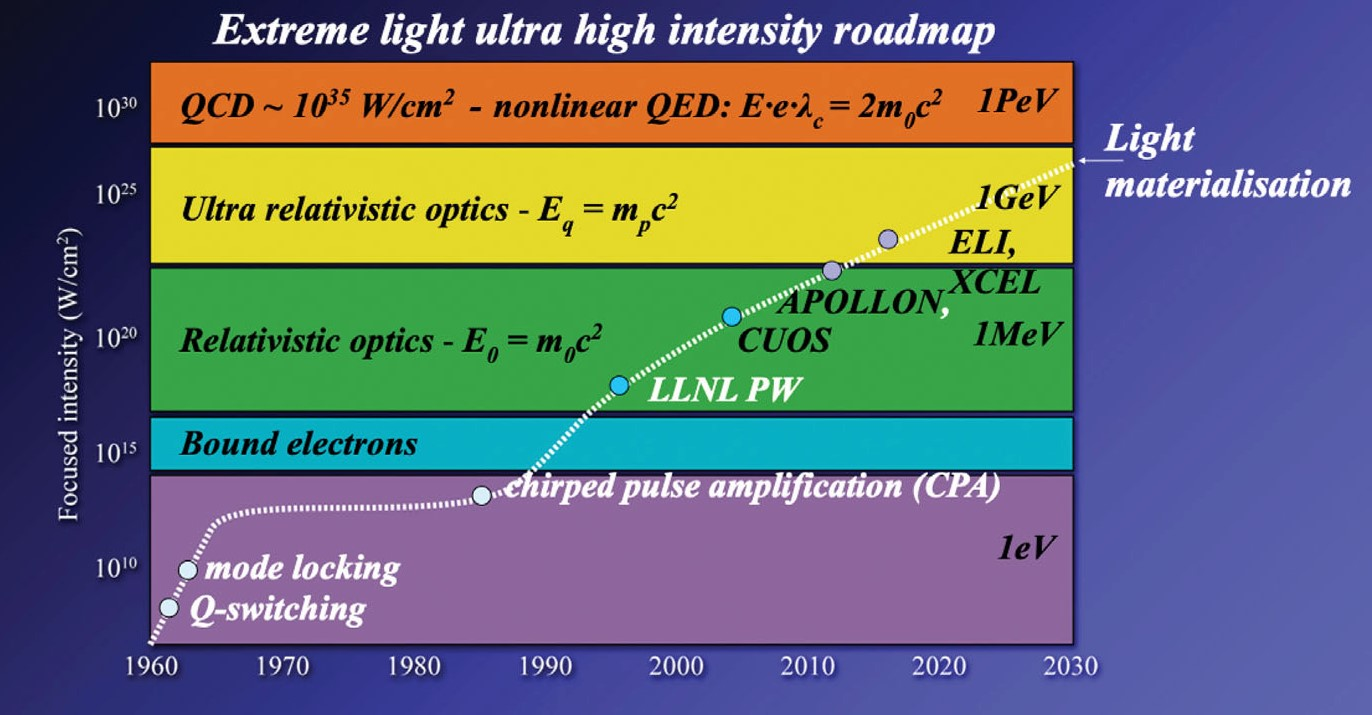
\includegraphics[width=0.8\linewidth]{figures/fig/fig1.1.jpg}
  \caption{激光发展史。}
  \label{tu1}
\end{figure}

如图~\ref{tu1}所示是激光发展史。激光强度小于$ 10^{14}~\mathrm{W/cm^{2}}$,此时激光所提供的电场强度不能够直接电离出原子中的束缚电子,此阶段强场物理研究激光与原子分子相互作用。激光强度处于$10^{14}~\mathrm{W/cm^{2}}\backsim 10^{18}~\mathrm{W/cm^{2}} $,激光的电场可以直接使得原子发生电离,形成等离子体,此阶段强场物理主要研究激光与等离子体相互作用。激光强度大于 $ 10^{18}~\mathrm{W/cm^{2}}$,使得我们对光与物质相互作用的研究进入了相对论非线性区域与非相对论性区域相比,激光场更有效地移动物质,粒子运动的高度非线性导致了很多新奇的物理现象,例如强激光场的Compton散射\cite{2018Compton},激光尾场加速\cite{2010wei},相对论自聚焦\cite{1974zi,1995zi}。

目前,激光强度达到了$ 10^{23}~\mathrm{W/cm^{2}}$的量级 \cite{2021jiguang},为了进一步提高激光强度,各地区正在建设的输出功率达到或超过10PW超高功率激光设施,如中国的极端光物理线站(Station of Extreme Light,SEL)\cite{2018SEL},法国的Apollon\cite{2015Apollon},欧盟的ELI(Extreme Light Infrastructure)\cite{2018ELI},美国的EP-OPAL(OMEGA EP-coupled Optical Parametric Amplifier Lines)\cite{2019OP},计划把激光强度达到$10^{23}~\mathrm{W/cm^{2}}\backsim 10^{24}~\mathrm{W/cm^{2}} $。对于强场量子电动力学(strong field quantum electrodynamics,SFQED)的探索,迫切需要激光强度超过$ 10^{23}~\mathrm{W/cm^{2}}$的超高功率激光器\cite{2019jiguan,2020jiguan}。在这个强度水平下,SFQED现象变得可观察;通过非线性康普顿散射(nonlinear Compton scattering, NCS)可以发射出超强的伽马射线,通过非线性布莱特-惠勒(Breit–Wheeler process,BW)过程可以产生电子-正电子对\cite{2006dzheng,2012zheng,2018zheng,2022zheng}。

\section{真空对产生}

根据Heisenberg的不确定性原理,我们知道在能量和时间上满足$\delta E \cdotp \Delta t \ge \frac{\hbar}{2}$,$\hbar$是普朗克常数。真空在极短时间内会有非常大的能量变化,对应着正负虚粒子的产生和湮灭。这就是真空涨落,2015年康斯坦茨大学的科研人员们直接验证了真空涨落现象的存在\cite{2015f},见图\ref{tu3}。这就是常说的“真空不空”,我们可以把真空看作是具有一定折射率和吸收率的极化介质。对于比较弱的外场,真空的结构非常稳定的,量子涨落所产生的虚粒子又很快湮灭掉而无法转换成实粒子。但在非常强的外场下,量子涨落所产生的虚粒子被强外场所拉开而不再发生湮灭,从而演化得到实粒子对,见图\ref{tu4}。在真空中能够产生一对正负电子对的临界电场可以通过在该电场下电场力把正负电子对拉开一个Compton波长的距离所做的功和电子的静止能量相等这一关系即$E_{\mathrm{cr}}=m^2c^{3} / e \hbar$估算出来,其中$m$是电子的静止质量,$c$是光速,$e$是电子电荷,

\begin{figure}
  \centering
  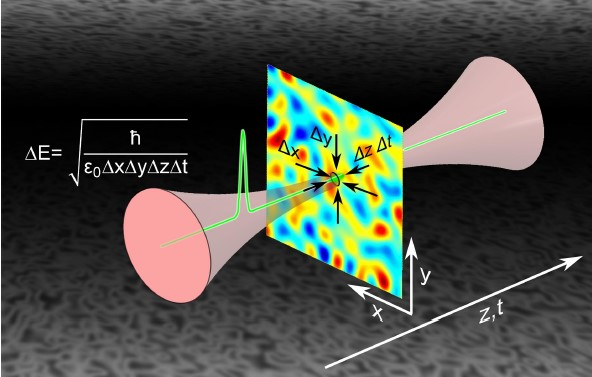
\includegraphics[width=0.8\linewidth]{figures/fig/fig1.3.jpg}
  \caption{真空涨落示意图}
  \label{tu3}
\end{figure}
\begin{figure}
  \centering
  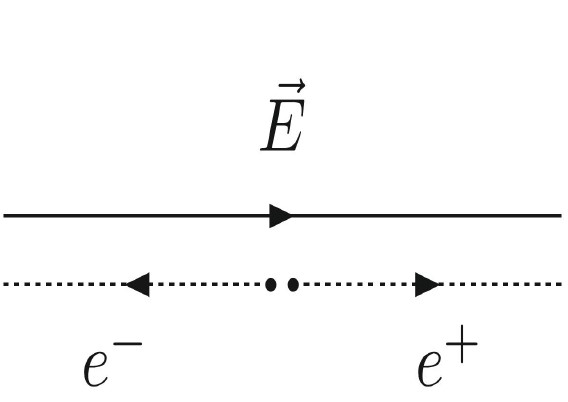
\includegraphics[width=0.8\linewidth]{figures/fig/fig1.4.jpg}
  \caption{强外场下真空产生正负电子对示意图}
  \label{tu4}
\end{figure}

随着激光强度的不断提高,光转化成物质是SFQED中的研究热点话题之一。由于需要对产生过程需要满足动量守恒和能量守恒,所以单个的平面波是不可能产生正负电子对。因此我们想要实现对产生,还需要在场中增加其他能量源来引发这个过程。有三种方法来实现对产生,见图~\ref{tu2}。(图(a)和(b)里的黑色实线代表Volkov正负能态,(b)中叉号顶点代表库仑场,(c)中的双线表示在驻波场中的电子传播子。如图~\ref{tu2}(a)所示是高能光子与强激光场中传播,高能光子与激光相互作用产生正负电子对。如图~\ref{tu2}(b)所示是激光在库仑场中传播,激光与原子核的库仑场相互作用产生正负电子对。如图~\ref{tu2}(c)所示,是利用两束激光对撞形成的驻波场来促进正负电子对的产生。

以上三种对产生机制,物理学家们已经在实验室实现了前两种。1996年,Bula等人使用斯坦福直线加速器(SLAC)产生的$46.6\mathrm{GeV}$的电子束和光子能量为$2.4\mathrm{eV}$,激光强度为$1.3 \times10^{18}~\mathrm{W/cm^{2}}$的强激光对撞验证了第一种正负电子对产生机制\cite{1996BW}。在这次电子与激光对撞实验中,科研人员利用多普勒效应,提高了在粒子静止系重点激光强度和激光频率,有效地促进了对产生过程。在该实验过程中,电子与激光光子对撞,发生NCS过程($e^- + n \omega_0 \to \acute e^- + \omega$),即产生了高能$\gamma$光子,频率为$\omega$。然后高能$\gamma$光子再与激光光子发生多光子Breit-Wheeler过程($\omega + n \omega_0 \to e^+ e^-$)产生正负电子对。

2010年,Chen等人利用$10^{20}~\mathrm{W/cm^{2}}$强激光照射金靶,在金靶后探测到正电子束\cite{2010BH},实现了第二种正负电子对产生机制,在实验过程中激光光子和金原子核发生散射产生高能$\gamma$光子,然后高能$\gamma$光子和高Z核发生Bethe-Heitler过程($Z+n \omega_{0} \rightarrow Z+e^{+}+e^{-}$)产生正负电子对。前面两种方式利用多普顿效应促进激光强度和频率在粒子静止系提升,从而增强对产生。第三种方式利用两束激光场对撞形成的驻波场来产生正负电子对,无法利用上述的机制来促进对产生,这样就导致需要的电场强度非常高,因此尚未在实验室中得到第三种机制产生正负电子对,这也是研究人员们一直在攻克的难题。

在下文中,我们对第三种正负电子对形成的不同机制(Schwinger机制和多光子过程)进行简要概述。为了形象化地表达物理本质,我们使用了一个经典的描绘真空状态的图像:狄拉克海图像。尽管我们知道这个图像已经过时,且与现代量子场论知识不兼容,但在许多方面,它仍然作为一个经典并且便于理解的物理模型存在。

\begin{figure}
  \centering
  \includegraphics[width=0.8\linewidth]{figures/fig/fig1.2.pdf}
  \caption{对产生三种过程的费曼图}
  \label{tu2}
\end{figure}

\subsection{Schwinger机制}

在真空中产生正负电子对是量子电动力学(quantum electrodynamics ,QED)中最有趣理论之一。1928年,Dirac在理论上预言了反物质存在\cite{1928s},具体来说,他预测了正电子的存在。Anderson的实验验证了这一预言,确凿无疑地证明了正电子的存在\cite{1933s}。1931年,Sauter提出产生真空中正负电子对这一问题\cite{1931s}。1936年,Heisenberg和Euler采用了有效拉格朗日量方法对对产生问题进行了进一步完善\cite{1936s}。到了1951年,Schwinger对真空对产生现象有了完整的理论描述\cite{1951s},为了纪念Schwinger在的卓越贡献,因此人们把在强场下真空通过隧穿效应产生正负电子对的过程成为Schwinger机制或者Schwinger效应。

一般来说,基本的物理思想是将真空状态视为一种材料,具有明显分离的导带(正能连续态)和价带(狄拉克海)。这两个带之间的带隙被假定为粒子和相应的反粒子的静止质量;在我们研究的情况下,是电子和正电子的质量。在真空状态下,正能连续态中没有电子,然而狄拉克海完全充满了具有负能量的电子。由于所有可观察的粒子必须具有正能量,因此我们观察不到狄拉克海的物质,例如有一束能量强至$2m c^{2}$的光子将狄拉克之海中的一个负能量电子提升为一个具有正能量的电子,那么在狄拉克之海中就会留下一个洞。这个洞相当于狄拉克之海中的一个粒子,它同时具有负能量态电子的所有相反属性,即具有正能量和正电荷。因此粒子创造的问题可以归结为将粒子从狄拉克海带到连续态的问题。由于这些带中的每一个空穴都可以与一个反粒子关联,所以上述的想法也同样适用于反粒子。

为了阐明导致电子对产生的各种机制,我们需要对真空态施加强电场。外部强场会使能带发生变形,如图\ref{tu5}所示,深蓝色能带代表着狄拉克海,浅红色能带代表着连续态。能带间隙(白色部分)是真实粒子禁止区域。。因此,从狄拉克海中激发电子到导带的各种情况变得可能。如果施加电场的场强是$E_{\mathrm{cr}}$的数量级,能带会发生强烈的变形,使电子可以从一个能带简单地隧穿到另一个能带。这种现象被称为施温格效应。如图\ref{tu6}展示了这样一个隧穿过程的示意图,当系统受到强电场作用时,能带会发生变形,使电子(黑点)可以隧穿到连续态。

\begin{figure}
  \centering
  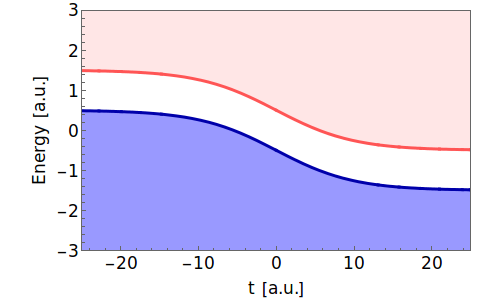
\includegraphics[width=0.8\linewidth]{figures/fig/fig1.5.png}
  \caption{强场下的能带图}
  \label{tu5}
\end{figure}

\begin{figure}
  \centering
  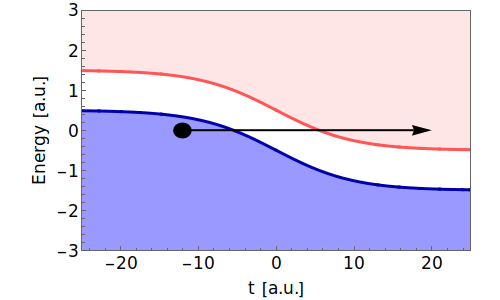
\includegraphics[width=0.8\linewidth]{figures/fig/fig1.6.png}
  \caption{施温格效应的图像描述}
  \label{tu6}
\end{figure}

下面我们来推导在Schwinger机制下的真空正负电子对的产生几率。从之前Sauter的工作中,在强电场下解狄拉克方程时,发现真空的正负能带在电场下会发生弯曲,对于足够大的电场强度,能级甚至可能发生交错。此时,根据量子隧道效应,负能带中的电子的将有一定概率隧道到正能带形成电子,同时在负能带中留下一个空穴,这个空洞就是电子的反物质-正电子的空穴理论。这就是量子力学中强场下真空生成正负电子对的物理图像。然后,可以从量子隧道的透射系数得到真空对生成的几率

\begin{equation}
    \mathcal{\Gamma}_{e^{-} e^{+}} \sim \exp \left(-\pi \frac{E_{\mathrm{cr}}}{|\mathbf{E}|}\right),
\end{equation}
其中,$E_{\mathrm{cr}}$为临界电场,$E$为外电场强度。

在Dunne的工作中\cite{2005L,2012L},对欧拉-海森堡拉格朗日量对理论物理的影响进行了回顾。欧拉-海森堡拉格朗日量通过非线性项扩展了麦克斯韦拉格朗日量,涵盖了在背景电磁场中产生的量子效应,表达式如下

\begin{equation}
 \mathcal L = \frac{e^2}{h c} \int_0^{\infty} \frac{d \eta}{\eta^3} e^{-\eta} \times \\
 { i\eta^2 {\mathbf{E} \cdot \mathbf{B}} 
 \frac{\cos {\frac{\eta}{E_0} \sqrt{\mathbf{E}^2 - \mathbf{B}^2 + 2 i{\mathbf{E} \cdot \mathbf{B}} }} +c.c}{\cos {\frac{\eta}{E_0} \sqrt{\mathbf{E}^2 - \mathbf{B}^2 + 2 i {\mathbf{E} \cdot \mathbf{B}} }} -c.c}
 + E_0^2 + \frac{\eta^2}{3} {\mathbf{B}^2 - \mathbf{E}^2} },
\end{equation}
其中,$ E_0 = \frac{m^2 c^3}{e \hbar} \approx 1.3 \ 10^{18} \ V/m$,$ E_0$首次在参考文献\cite{1931s}中确定,被定义成在真空在恒定电场下创造物质的临界场强。通过对弱场进行摄动展开拉格朗日量,可以获得对麦克斯韦拉格朗日量的主要量子修正

\begin{equation}
\mathcal{L}_{pert}  = \frac{\mathbf{E}^2 - \mathbf{B}^2}{2} + \frac{1}{90 \pi} \frac{\hbar c}{e^2} \frac{1}{E_0^2} { {\mathbf E^2 - \mathbf B^2}^2 + 7 {\mathbf{E} \cdot \mathbf B}^2}.
\end{equation}
值得注意的是,拉格朗日量完全是以洛伦兹不变量的形式构建的
\begin{equation}
\mathcal F = -\frac{1}{4} F^{\mu \nu} F_{\mu \nu} = \frac{1}{2} {\mathbf{E}^2 - \mathbf{B}^2} ,\qquad \mathcal G = -\frac{1}{4} F^{\mu \nu} \tilde F_{\mu \nu} = \mathbf{E} \cdot \mathbf{B}
\end{equation}
其中,第二项被临界场强$E_0$抑制。

在发展重整化方案并将其纳入量子电动力学以形成电磁力的完全协变表述的过程中,利用新技术进一步研究了对产生问题。将对产生过程视为适当时空的演化过程\cite{1951s}, Schwinger能够将物质的创造与恒定场的有效拉格朗日量联系起来
\begin{equation}
 \mathcal L = \frac{1}{2} E^2 - \frac{1}{8 \pi^2} \int_0^{\infty} \frac{ds}{s^3} \left ( {e E \ s \ \text{cot} {\left ( e E \ s \right ) } - 1 + \frac{1}{3} {\left ( e E \ s \right ) }^2}\right ). 
\end{equation}
它的虚部特别重要
\begin{equation}
    \text{Im} \ \mathcal L = \frac{\alpha^2}{2 \pi^2} E^2 \sum_{n=1}^{\infty} n^{-2} \exp {\frac{-n \pi m^2}{e E}}.
\end{equation}
以上描述了恒定电场中真空衰变速率。此外,这个求和的第一项给出了单个电子-正电子对的产生率:
\begin {equation} \label{NS}
 \dot N = \frac{\alpha^2}{2 \pi^2} E^2 \exp {\frac{- \pi m^2}{e E}}.
\end {equation} 

\subsection{多光子过程}

第二种机制是电子通过吸收高能光子而激发。在这种情况下,电子吸收了光子的能量,导致电子的净能量足够克服带隙(见图\ref{tu7}左);如果同时吸收了多个光子,我们称这种效应为多光子对产生(见图\ref{tu7}右)。图\ref{tu7}是一个关于多光子吸收的描述图,其中一个电子同时吸收$n$个光子。在左侧,一个高能光子被狄拉克海(深蓝色区域)中的电子(黑点)吸收。电子的最终能量足够高,以克服带隙(白色区域)并达到连续体(浅红色区域)。有时,单个光子的能量可能不足以产生一个粒子对。因此,右侧显示了一个$n = 2$的吸收过程。

\begin{figure}
  \centering
  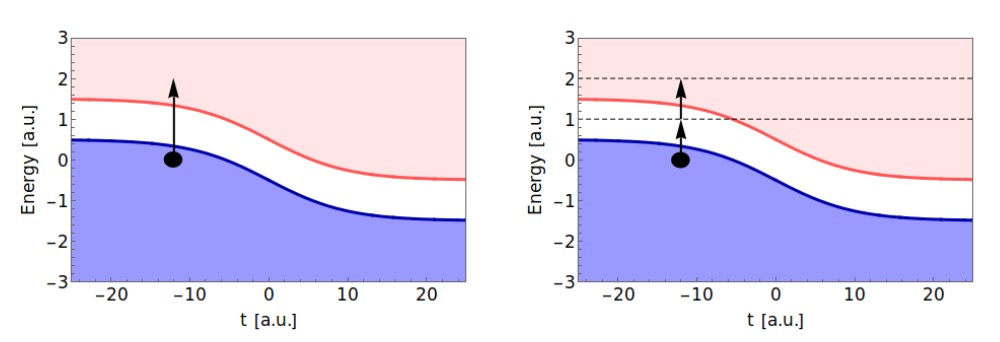
\includegraphics[width=0.8\linewidth]{figures/fig/fig1.7.jpg}
  \caption{多光子吸收示意图}
  \label{tu7}
\end{figure}

在这里,我们就不花费较长篇幅去推导多光子机制下的真空对产生率,而选择直接给出表达式:
\begin{equation}\label{ND}
 \dot N \approx \begin{cases}  \exp \left(\-\frac{\pi m^2 c^3}{e \hbar E}\right), & \gamma \ll 1 \\ (\frac{e E}{2m \omega})^{4mc^2/ (\hbar \omega)}, & \gamma \gg 1\end{cases}.
\end{equation}
其中$E$为外加电场强度,$\omega$为电场频率,$m$为电子的静止质量,$c$是光速,$\gamma$是Keldysh参数。Keldysh参数可以用来评估在对产生过程中是隧穿过程主导还是多光子吸收过程主导,定义如下:
\begin{equation}\label{Keldysh3}
 \gamma = \frac{m \omega}{e E}.
\end{equation}
此外,假设一个$n$光子吸收过程导致对产生,那么$n+m$光子过程的机会是非零的。由于$n$,$m$是任意的非负整数,这必然在相空间中产生一个明显的特征,因为产生的粒子的动量有所不同。类似于大家熟知的原子电离中的过程,我们把这种效应被称为超阈值对产生(见图\ref{tu8})。从最新的理论计算研究所知道到的,还有一种组合效应的可能性。如果电子吸收的光子能量不足以将电子推向连续体,那么还有两种可能情况。电子要么以光子的形式发射能量,重新回到狄拉克海;要么从虚态通过隧穿效应跃迁到连续体。这种动力学辅助的施温格效应的原理在图\ref{tu8}中有所说明。

\begin{figure}
  \centering
  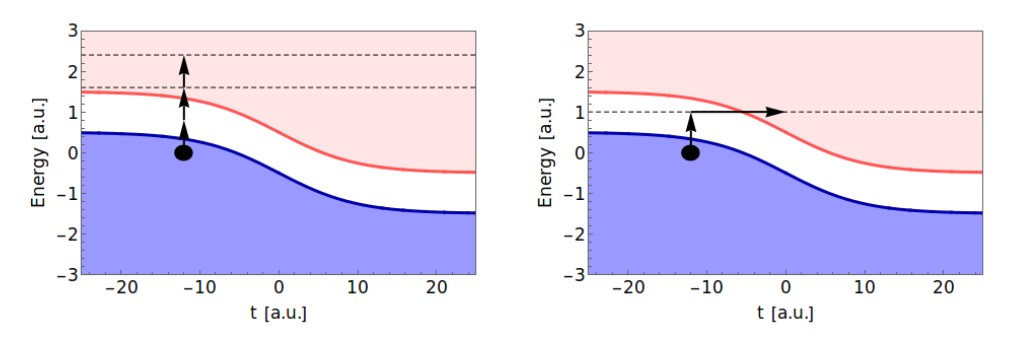
\includegraphics[width=0.8\linewidth]{figures/fig/fig1.8.jpg}
  \caption{超阈值对产生和动力学辅助的Schwinger机制示意图}
  \label{tu8}
\end{figure}

\section{研究现状}

考虑到当前激光的空间聚焦尺度远大于产生正负电子对所需的空间尺度(即电子的康普顿波长),由两束激光碰撞形成的驻波场可以被视为随时间变化的空间均匀电场。在此场下的粒子对生成问题实际上是将对产生问题推广到含时间电场的情况,研究的重点主要在于优化外部场构型以降低粒子对生成的阈值和提高对的产量,以及研究复杂强场下粒子对生成的性质。在各种复杂强外场中的真空对产生问题已经得到了广泛而深入的研究。这些复杂强外场包括由慢变强场和快变弱场组成的组合场,具有脉冲形状不对称的不同极化场,以及频率啁啾场。在这些不同配置的外场下,真空正负电子对生成过程呈现出许多新的现象,如动力学辅助下的对产生,动量谱的振荡,以及多峰干涉效应。以下给出了在不同场配置下的对生成过程中的一些重要结果,这将有助于理解本论文的主要工作。

\subsection{动力学辅助的Schwinger机制}

从公式\ref{NS}我们可以知道在弱电场下,正负粒子对的产生率呈指数级抑制,因此,用当前的激光场强度观察施温格机制对产生过程非常困难。此外,从公式\ref{ND}可以看出,多光子区域下低频激光场中的粒子对生成率也大致呈指数级抑制。因此,在目前的激光条件下仅由这两种对生成机制产生的粒子数量将非常少,于是自然而然的想到,能不能将这两种机制结合起来,来促进对的产生,我们把这结合机制叫做动力学辅助的Schwinger机制,原理可以在图\ref{tu8}右测得到一个清晰的解释。2008年Sch{\"u}tzhold等人就创造性地完成了这个工作\cite{2008d},他们的研究主要关注由强而缓慢变化的电场(施温格效应)诱导的正负电子对对从狄拉克真空中的产生,同时这个电场又被一个弱而快速变化的电磁场(动力学对产生)所叠加。在亚临界区域,这两种机制单独作用时都会被强烈抑制,但当它们联合作用时,会显著增强对生成率。强电场降低了动态粒子生成的阈值,快速的电磁场为施温格机制提供了额外的“可能”。

\subsection{脉冲形状不对称对对产生的影响}

2014年,Obulkasim等人通过量子Vlasov方程(quantum Vlasov equation, QVE) ,研究了强非对称激光电场中的电子-正电子对产生\cite{2014as}。该研究考虑了亚周期、周期和超周期激光脉冲的三种不同情况。在非对称激光脉冲场中,其中一个上升或下降侧的脉冲长度固定,而另一侧的脉冲长度改变,与对称情况相比,对产生率和数密度可以显著修改。对于这三种不同周期脉冲的每一种情况,当一侧脉冲长度恒定,另一侧脉冲长度变短(即整个脉冲被压缩)时,可以产生比相反情况(即整个脉冲被拉长)更多的对。在压缩脉冲的情况下,存在一种最优的非对称脉冲长度比,使得对数密度最大。此外,由亚周期脉冲产生的最大对数密度大于周期和/或超周期脉冲产生的对数密度。然而,在拉长脉冲的情况下,只有对于超周期激光脉冲,产生的对增强,并且也存在一种最优的非对称脉冲长度比,使得对数密度最大。另一方面,令人惊讶的是,在亚周期和周期拉长激光脉冲的两种情况下,随着脉冲的不对称性增加,对数密度单调递减。2020年,他们再使用 Dirac–Heisenberg–Wigner(DHW)方法,研究了极化电场中非对称脉冲对对产生的影响\cite{2020as}。研究探究了在三种典型的极化场:线极化,椭圆极化和圆极化场中正负电子对的生成。研究了下降脉冲长度的两种不对称性,缩短和延长。研究发现,随着脉冲长度的缩短,干涉效应消失,动量谱的峰值集中在动量空间的中心。在延长下降脉冲长度的情况下,动量谱中出现了无干涉的多环结构。研究结果显示,动量谱对脉冲的不对称性以及场的偏振非常敏感。还发现,不同偏振下的粒子的数密度对电场的不对称性敏感。对于短下降脉冲,数密度可以显著增强,超过两个数量级。

\subsection{频率啁啾对正负电子对产生的影响}

首先,我们介绍在空间均匀含时电场中频率啁啾对正负电子对产生的影响。2010年,Dumlu在啁啾激光脉冲的背景下\cite{2010c},研究已经分析了这些具有子周期结构的脉冲,并研究了啁啾参数对产生粒子的动量谱的影响。也分析了啁啾和激光脉冲的载波相位的联合效应。通过在复WKB散射方法对产生对的框架内研究势的转折点结构,定性地解释了这些效应。2013年,姜敏等人根据QVE方法,研究了频率啁啾对电子对生成的影响\cite{2013cj}。同时也考虑了周期参数,该参数表征了脉冲内激光场的周期度。在超周期和子周期激光脉冲中,频率啁啾都可以大大增强产生的对的动量分布函数和对的数密度。由超周期激光脉冲产生的对数密度大于在相同的激光频率和啁啾下由子周期脉冲产生的对数密度。对于不同的啁啾率,存在一个对应于产生的对数密度最大值的最佳周期参数。发现当周期参数低于/高于最佳值时,对数密度对啁啾率敏感/不敏感。同年,李子良等人同样运用QVE的方法研究频率变化对强脉冲激光场中真空对产生的影响\cite{2013cl}。他们发现,缓慢变化的频率可以在一定程度上影响对产生,而快速变化的频率可以在时间位于一个窄时间窗口内(在此窗口中发生频率跳跃)时,将对创建率增加几个数量级。对增强对现象背后可能的物理机制也进行了简要讨论。

2017年,Nuriman等人利用QVE方法研究了双色的频率啁啾场\cite{2017c}。他们探究了在一色和二色激光脉冲场中,通过频率啁啾产生电子对的过程。频率啁啾是指信号频率随时间的变化,在这里,它被用来调制激光脉冲。研究发现,小的频率啁啾可以沿着动量轴移动动量谱。在二色脉冲场中产生的对的数密度远高于一色脉冲场中的数密度。通过与固定频率的比较,发现频率调制对电子数量有显著的增强效应。特别是当频率较小时,适当的频率调制可以增强对产生中的多光子过程,从而促进对的产生。2019年,Obulkasim等人利用DHW方法研究在频率啁啾的不同极化电场中的对产生\cite{2019c}。他们使用实时的DHW形式来研究电场,将其模型化为具有亚临界峰值场强的均匀单脉冲场。他们计算了四种不同极化(线极化、椭圆极化、近圆椭圆极化和圆极化)以及一些线性频率啁啾的动量谱。他们发现频率啁啾导致了强烈的干涉效应和动量谱的显著变化,具体取决于所选的极化。产生的对的数密度非线性地依赖于表征极化的参数,并且对啁啾参数的变化非常敏感。对于一些研究过的频率啁啾,这可以提供三到四个数量级的数密度增强。2020年,龚弛等人使用QVE方法研究了频率调制激光场中产生的电子-正电子对的动量谱和数密度\cite{2020cg}。动量谱呈现出明显的干涉模式,这是频率调制场在动量谱上的印记,因为动量峰值对应于通过吸收不同频率组分的光子的对产生过程。此外,通过分析转折点结构,也可以定性地理解干涉效应。对数密度的研究表明,数密度对调制参数非常敏感,对于某些调制参数,可以增强2到3个数量级。2021年,王焜等人研究了对称频率啁啾效应对对产生的影响\cite{2021cw}。他们研究使用了DHW形式来研究在对称频率啁啾的电场的线、椭圆、近圆和圆极化下的电子对产生,并得到动量谱和对产量。他们发现,对于小的啁啾,极化场之间的结果差异是明显的。当啁啾参数增加时,动量谱倾向于展示由多同心环结构表征的多光子对生成。与非对称频率啁啾的情况相比,数密度的增加也非常显著。与非对称频率啁啾的情况相比,数密度的增加也非常显著。他们指出,动力学辅助的施温格机制在对称频率啁啾中增强对产生中起着重要作用。

接下来,我们再来介绍对于空间和时间都依赖的电场,我们看看频率啁啾效应如何影响对产生。2020年,Mamutjan等人研究了空间非均匀振荡电场中的啁啾效应对电子对产生的影响\cite{2020cm}.他们使用了DHW形式来研究非均匀电场下真空对产生的啁啾效应,发现对于快速振荡的电场,粒子动量谱对空间尺度和啁啾参数都敏感。对于最大的啁啾,外部场宽度的影响较小。对于慢速振荡的电场,大的空间范围内可以识别出啁啾效应,载波相位在小的空间尺度上也能显著反映出啁啾效应。在准均匀极限下,所有考虑的外部场配置都满足局部密度近似,允许人们使用来自均匀场的方法来分析非均匀场结果。2021年,Melike等人继续用DHW方法研究对称频率啁啾在不均匀电场中\cite{2021cMM}。他们研究了高频和低频模式,并考虑了两个载波包络相位。发现动量谱对啁啾敏感,导致对于不同的空间尺度以及外部场的载波相位产生不同的干涉效应。随着啁啾的增加,约化的粒子数通常会增强。也研究了场的空间尺度对减少粒子数的影响。发现在小的空间尺度上,它会增强,但在大的空间尺度上,对于考虑的场参数,它几乎不会改变。在小的空间尺度上,当应用啁啾时,约化粒子数会增强一个或两个数量级,除了余弦低频场,它只是大几倍。此外,发现通过与高频场中通常的非对称啁啾比较,对称啁啾进一步增加了约化粒子数,大约增加了两倍。同年李烈娟等人利用DHW形式来研究啁啾参数对单一场或动态辅助组合场在各种空间尺度下的约化动量谱和总粒子产量的影响\cite{2021cL}。对于单一高频场和组合场,随着啁啾的增加,动量谱的干涉效应变得更加显著。在有啁啾的动力学辅助场情况下,当两个场存在啁啾时,约化的总产量显著增强。具体来说,在动力学辅助场情况下,当应用啁啾时,小空间尺度上的减少粒子数增加了一个或两个数量级,而在大空间尺度上,它增强了大约两倍。该研究还为各种情况下的总产量和增强因子提供了一些最优的啁啾和空间尺度参数。

2023,Melike等人研究了载波包络相位对在具有对称频率啁啾的空间非均匀电场中的产生的影响\cite{2023cMM}。在高频和低频场中,他们发现由相位引起的动量谱和减少的粒子数都有周期性的变化。特别地,在低频场的情况下,这些变化更为敏感。在某些条件下,由相位引起的减少的粒子数可以增加一个数量级以上他们在动量谱中揭示了两个相关相位的一些不同类型的对称性和一个有趣的个体自对称性。相位和啁啾的联合作用在动量谱和减少的粒子数的周期性和对称性行为中提供了更灵活的参数选择,以控制和优化对产生。同年,Emin等人研究了电场啁啾对不同振荡电场中对产生的影响\cite{2023ce}。该研究主要考虑了二次和正弦啁啾电场。结果表明,啁啾显著影响了由低频隧道效应主导的电场中产生的粒子的动量谱,特别是在正弦啁啾场中,动量谱的振荡明显。然而,随着啁啾参数的增加,多光子过程逐渐显现。因此,在由多光子过程主导的高频电场中,生成粒子的数密度随着在二次啁啾场中的啁啾参数的增加而增加,而动量分布保持相对对称。在正弦啁啾电场中,引入啁啾参数立即改变了动量分布,导致对称性的破坏。此外,存在一个最优的啁啾参数,在正弦啁啾电场中,总粒子数在最优啁啾下增加了大约一个数量级以上;超过一定的阈值后,产生的粒子的数密度减少,表明在正弦电场中啁啾有抑制效应。同年,王莉等人使用计算量子场论(CQFT)研究了线性啁啾频率下复合势阱中正负电子对对增强。在适当的啁啾参数下,复合势阱下产生的电子对数量可以增加两到三倍。在低频区域,频率调制激发了干涉效应和多光子过程,这促进了电子对的生成。在高频区域,高频抑制抑制了电子对的生成。对于单个势阱,在低频区域,产生的电子对的数量可以提高几个数量级。有趣的是,胡丽娜等人还利用频率啁啾来调制相位研究了在空间非均匀电场中带有正弦相位调制的电子对产生\cite{2023ch}。重点讨论了调制参数对动量谱和各种空间尺度下的约化粒子数的影响。对于动量谱,随着调制幅度或频率的增加,干涉效应变得越来越显著,而当调制幅度时,对称性被严重破坏。对于减少的粒子数,当应用调制参数时,它会大约增加几倍,甚至一个数量级。此外,研究了空间尺度对约化粒子数的影响,发现它在小的空间尺度上迅速增加,而在大的空间尺度上趋于常数。我们还得到了可以通过不同的调制实现的最优对产生。这些结果为通过结合场的空间非均匀性和不同的相位调制选择来实现最优对产生提供了可能性。

\section{本论文的主要研究内容}
本论文采用DHW形式,对频率啁啾场下的真空正电子-负电子对问题进行了深入研究。通过对得出的结果进行详细的分析和讨论,我们进一步深化了对粒子对生成机制的理解。以下是本论文的主要工作和结构:
第2章主要介绍DHW形式。
第3章采用实时的DHW形式,研究了不对称脉冲形状在场中对电子-正电子对产生的影响进行了深入探讨,涵盖了三种不同的啁啾情况。分析了产生粒子的动量谱和数密度。
第4章研究对称频率啁啾电场对电子对产生的影响。
第5章对论文内容进行总结与展望。






% !TeX root = ../bnuthesis-example.tex

\chapter{DHW形式}
早期常用的研究真空对生成问题的方法包括有效作用量、固有时间方法和Wentzel-Kramers-Brillouin (WKB) 近似。已经开发出许多更简单、更实用的半经典近似和量子动力学方法,包括世界线瞬子技术 (worldline instantons,WI) ,S矩阵(S-matrix),量子Vlasov方程 (QVE) 和 Wigner函数形式\cite{2017xie}。DHW 形式不仅可以用来研究在存在空间非均匀含时电场的情况下的真空对生成问题,也可以用来研究在存在磁场的情况下的对生成过程。事实上,DHW形式可以理论上研究在任何类型的电磁场下的真空对生成问题。然而,对于高维场,它通常受到计算机存储大小和计算能力的限制。值得注意的是,对于空间均匀含时电场,DHW 形式可以简化为QVE。在众多关于在电子对真空中生成正负电子对的方法中,本论文选择了DHW形式。这种方法起始于狄拉克密度算符,引入了维格纳函数,最终导出了完整的DHW运动方程。由于关于DHW形式的推导众多且复杂,本文在这里仅仅对空间均匀含时电场下的DHW形式做简单介绍。

\section{Winger算符}

量子力学的相空间表述最初是为了研究经典统计力学的量子修正而引入的,其中,维格纳函数是为此目的引入的最著名的相空间表述之一。相空间表述的优点不仅在于它提供了一种用经典语言描述量子系统的方式,而且还揭示了粒子运动的实时动态。如今,维格纳函数广泛用于处理非相对论量子物理问题。

维格纳函数的形式是建立在厄米QED拉格朗日量的基础上的:
\begin{equation}
    \mathcal{\hat{L}}(\hat{\Psi},\bar{\hat{\Psi } },\hat{\overrightarrow{A} } ) = \frac12\left[\bar{\hat{\Psi }}\gamma^\mu [i \partial_\mu-eA_\mu]\hat{\Psi}-\left([i\partial_\mu+eA_\mu]\bar{\hat{\Psi }}\right)\gamma^\mu\hat{\Psi}\right]-m\bar{\hat{\Psi }}\hat{\Psi}-\frac14F^{\mu\nu}F_{\mu\nu},
\end{equation}
由此得到旋量的狄拉克方程$\hat{\Psi}$及其伴随旋量的伴随形式 $\bar{\hat{\Psi}}=\hat{\Psi}^\dagger\gamma^0$,并且
\begin{equation}
\begin{aligned}
&\partial_{t} \hat{\Psi}(\vec{x}, t)=-\gamma^{0} \vec{\gamma}\left[\vec{\nabla}_{\vec{x}}-i e \hat{\vec{A}}(\vec{x}, t)\right] \hat{\Psi}(\vec{x}, t)-i m \gamma^{0} \hat{\Psi}(\vec{x}, t) \\
&\partial_{t} \overline{\hat{\Psi}}(\vec{x}, t)=-\left[\nabla_{\vec{x}} \hat{\hat{\Psi}}(\vec{x}, t)+i e \hat{\hat{\Psi}}(\vec{x}, t) \hat{\vec{A}}(\vec{x}, t)\right] \cdot \vec{\gamma} \gamma^{0}+i m \hat{\hat{\Psi}}(\vec{x}, t) \gamma^{0}
\end{aligned}        
\end{equation}
注意,这里使用了爱因斯坦的求和约定。电磁场将被视为一个经典的外场,它的运动方程将被简化为$\vec{E}$和$\vec{B}$服从麦克斯韦方程的要求:
\begin{equation}
\operatorname{div} \vec{E} = \rho \quad \operatorname{rot} \vec{E} = -\dot{\vec{B}} \quad
\operatorname{div} \vec{B} = 0 \quad \operatorname{rot} \vec{B} = \dot{\vec{E}}+\mu_{0} j .
\end{equation}
从费米子场算子$\hat{\Psi}$及其共轭算子$\hat{\Psi}^\dagger$出发,
\begin{equation}
C_{ab}^{\pm}(t,\vec{x_{1}},\vec{x_{2}}):=\langle0|\hat{\Psi}_{a}(t,\vec{x_{1}})\hat{\Psi}_{b}^{\dagger}(t,\vec{x_{2}})|0\rangle\pm\langle0|\hat{\Psi}_{b}^{\dagger}(t,\vec{x_{2}})\hat{\Psi}_{a}(t,\vec{x_{1}})|0\rangle,
\end{equation}
可以用来建立维格纳函数。由于$C^+$是域算子的反对易子的期望值,根据定义它是$\delta_{ab}\cdot\allowbreak\delta(\vec{x_2}-\vec{x_1})$函数,所以只有$C^-$包含非平凡信息。因此,场算符的换向子将是维格纳函数定义中的起点。引入实验室坐标系质心坐标$\vec{x}$,相对坐标$\vec{s}$ 
\begin{equation}
     \vec{x} : =  \frac12\left( \vec{x_1} + \vec{x_2} \right) \\
  \vec{s} : = \vec{x_2} - \vec{x_1}\,.
\end{equation}
现在,Wigner算子$\hat{\mathcal{W}}$被定义为Heisenberg图中两个Dirac场算子的等时间密度算子的傅里叶(Wigner)变换。由于我们对真空的对产生感兴趣,Wigner函数是通过取Wigner算子的真空期望值来定义的$\langle0|\diamond|0\rangle $。注意使用Dirac共轭场算子$\bar{\hat{\Psi} }=\hat{\Psi}^\dagger\gamma^0$代替伴随场算子,使得Wigner算子在洛伦兹变换下齐次变换

\begin{equation}\label{2-6}
 \begin{aligned}
&\mathcal{W}(t,\vec{x},\vec{p}) :=\langle0|\hat{\mathcal{W}}(t,\vec{x},\vec{p})|0\rangle   \\
& \hat{\mathcal{W}}_{ab}(t,\vec{x},\vec{p}):=-\frac12\int d\overrightarrow{s}\mathrm{~e}^{-\frac{\mathrm{i}}\hbar\vec{p}\cdot\vec{s}}\hat{\mathcal{C}}_{ab}(t,\overrightarrow{x},\overrightarrow{s})  \\
&\hat{\mathcal{C}}_{ab}(t,\vec{x},\vec{s}) :=\hat{\Phi}(t,\vec{x},\vec{s})\left[\hat{\Psi}_{a}(t,\vec{x}+\vec{s}/2),\overline{\hat{\Psi}_{b}}(t,\vec{x}-\vec{s}/2)\right]  \\
&\hat{\Phi}(t,\vec{x},\vec{s}) :=\mathcal{P}\text{e}^{-\mathrm{i}e\int_{\vec{x}+\vec{s}/2}^{\vec{x}-\vec{s}/2}\vec{\hat{A}}(t,\vec{x}^{\prime})\cdot d\vec{x}^{\prime}} .
\end{aligned}
\end{equation}

引入Wilson线因子$\hat{\Phi}(t,\vec{x},\vec{s})$来实现规范不变性。
对电磁场进行经典处理后,路径排序将被去掉。选择一条直线作为积分路径,可以保证对$\vec{p}$作为动能的正确解释。请注意,这不是依赖于时空点和四动量的协变维格纳函数的定义,而是取能量平均值的等时维格纳函数。傅里叶变换可以理解为测量两点相关相对于原点$\vec{x}$的平面波含量。然后将平面波的振幅解释为在位置 $\vec{x}$处动量为$\vec{p}$的粒子的准概率密度。因此Wigner函数可用于计算期望值任何可观察到的,用场算符表示的。如果将变量$\vec{x}$或$\vec{p}$ 中的一个积分出来,则剩余的函数为正,可以解释为粒子密度。

\section{运动方程}

在定义方程式\ref{2-6} 中,对每个场算符使用海森堡运动方程,可以推导出 Wigner函数的运动方程。结果是一个耦合方程组,它不仅描述 Wigner函数的演化,还描述了电磁场的演化。这个被称为 BBGKY方程组,以 N. Bogoliubov、M. Born、H.Green、G. Kirkwood 和 J.Yvon 的名字命名。为了进行实际的数值计算,这个方程组可以被截断。这种Hartree 型或平均场近似,将在下面解释,实际上是到目前为止在 Wigner 方法中使用的唯一近似。

我们用期望值的乘积来代替算子的期望值
\begin{equation}
 \begin{aligned}
&\langle 0|\hat{E} \hat{\mathcal{O}}| 0\rangle \rightarrow\langle 0|\hat{E}| 0\rangle \cdot\langle 0|\hat{\mathcal{O}}| 0\rangle, \\
&\langle 0|\hat{B} \hat{\mathcal{O}}| 0\rangle \rightarrow\langle 0|\hat{B}| 0\rangle \cdot\langle 0|\hat{\mathcal{O}}| 0\rangle .
\end{aligned}
\end{equation}

BBGKY层次结构的无穷方程组在Wigner函数的第一能级和电磁场的第零能级被截断,因为后者被视为经典背景场。然后可以将Wigner函数的动力学方程写成:
\begin{equation}\label{2-8}
    D_t\mathcal{W}=-\frac12\vec{D}_{\vec{x}}\left[\gamma^0\vec{\gamma},\mathcal{W}\right]-\mathrm{i}m\left[\gamma^0,\mathcal{W}\right]-\mathrm{i}\vec{P}\left\{\gamma^0\vec{\gamma},\mathcal{W}\right\}
\end{equation}
其中伪微分算子
\begin{equation}
 \begin{aligned}
&D_{t} =\partial_{t}+e\int\limits_{-1/2}d\lambda\vec{E}(t,\vec{x}+\mathrm{i}\lambda\vec{\nabla}_{\vec{p}})\cdot\vec{\nabla}_{\vec{p}}, \\
&\vec{D}_{\vec{x}} =\vec{\nabla}_{\vec{x}}+e\intop_{-1/2}^{1/2}d\lambda\vec{B}(t,\vec{x}+\mathrm{i}\lambda\vec{\nabla}_{\vec{p}})\times\vec{\nabla}_{\vec{p}}, \\
&\vec{P} i=\vec{p}-\mathrm{i}e\int\limits_{-1/2}^{1/2}d\lambda\lambda\vec{B}(t,\vec{x}+\mathrm{i}\lambda\vec{\nabla}_{\vec{p}})\times\vec{\nabla}_{\vec{p}}. 
\end{aligned}
\end{equation}
在这里,我们使用约定$\left \{  {\gamma^\mu}{\gamma^\nu} \right \}=+2\eta^{\mu\nu}=+2\operatorname{diag}(1,-1,-1,-1)$和使用时间规范$A_0=0$。电场$\vec{E}$和磁场$\vec{B}$由下式给出:
\begin{equation}
    \begin{aligned}\vec{E}&=-\partial_t\vec{A}\\\vec{B}&=\vec{\nabla}_{\vec{x}}\times\vec{A}.\end{aligned}
\end{equation}
在费曼图的语言中,平均场近似对应于忽略辐射修正,这是由精细结构常数 
$\alpha$很小所导致的。Wigner函数可以用Dirac双线性函数的完备基进行分解$(\mathbb{1},\gamma^5,\gamma^\mu,\gamma^\mu\gamma^5,\sigma^{\mu\nu}:=\frac{\mathrm{i}}{2}\left[\gamma^\mu,\gamma^\nu\right])$,
\begin{equation}\label{2-11}
\mathcal{W}=\frac14\left(\mathbb{1}\text{s}+\text{i}\gamma_5\text{p}+\gamma^\mu\text{v}_\mu+\gamma^\mu\gamma_5\text{al}_\mu+\sigma^{\mu\nu}\text{t}_{\mu\nu}\right)
\end{equation}
与相应的变换系数函数$\mathbb{s},\mathbb{p},\mathbb{v_\mu},\mathbb{a_\mu},\mathbb{t_{\mu\nu}}$。将方程\ref{2-11}代入方程\ref{2-8},后者可以分解,得到
\begin{equation}\label{2-12}
\begin{aligned}
&D_{t} s=\quad+2 \vec{P} \cdot \overrightarrow{\mathbb{t}}^{1} \\
&D_{t} \mathbb{P}=\quad-2 \vec{P} \cdot \overrightarrow{\mathbb{t}}^{2}-2 m \mathrm{a}^{0} \\
&D_{t} \mathbb{\mathbb { v }}^{0}=-\vec{D}_{\vec{x}} \overrightarrow{\mathbb{v}} \\
&D_{t} \mathrm{a}^{0}=-\vec{D}_{\vec{x}} \vec{a} \quad+2 m \mathbb{p} \\
&D_{t} \overrightarrow{\mathbb{V}}=-\vec{D}_{\vec{x}} \mathbb{v}^{0} \quad-2 \vec{P} \times \vec{a}-2 m \overrightarrow{\mathbb{t}}^{1} \\
&D_{t} \overrightarrow{\mathrm{a}}=-\vec{D}_{\vec{x}} \mathrm{a}^{0} \quad-2 \vec{P} \times \overrightarrow{\mathrm{v}} \\
&D_{t} \overrightarrow{\mathbb{t}}^{1}=-\vec{D}_{\vec{x}} \times \overrightarrow{\mathbb{t}}^{2}-2 \vec{P}\mathbb{s} \quad+2 m \overrightarrow{\mathbb{v}} \\
&D_{t} \overrightarrow{\mathbb{t}}^{2}=+\vec{D}_{\vec{x}} \times \overrightarrow{\mathbb{t}}^{1}+2 \vec{P} \mathbb{p} \\
\end{aligned}
\end{equation}
两个向量$\vec{\mathbb{t}}^{1/2}$包含了反对称张量的分量 ${\mathbb{t}}_{\mu\nu}$

\begin{equation}
\vec {\mathbb{t}}^{1} : = 2 \mathbb{t}^{i0}\vec{e_i},  
\vec {\mathbb{t}}^{2} : = \mathbb{t}_{ij}\epsilon^{ijk}\vec{e_k}\,.
\end{equation}
当时间$t\to -\infty$,$\vec{E}$ and $\vec{B}$ 逐渐消失,初始条件由具有非零分量的真空解给出

\begin{equation}\label{2-14}
\mathbb{s}_{\mathrm{vac.}}=\frac{-2m}{\omega(\vec{p})},
\mathbb{v}_{\mathrm{vac.}}=\frac{-2\vec{p}}{\omega(\vec{p})},
\end{equation}
其中$\omega^2: = \vec{p}^2+m^2$.
真空解也可以用矩阵形式写成:
\begin{equation}
\mathcal{W}_{\mathrm{vac}}=\frac14(\mathbb{1}\mathbb{s}_{\mathrm{vac}}+\gamma^\mu\mathbb{V}_{\mathrm{vac}\mu})=-\frac m{2\omega}\mathbb{1}+\frac{\vec{\gamma}\cdot\vec{p}}{2\omega}.
\end{equation}
运动方程式\ref{2-12}结合初始条件式\ref{2-14}定义初值问题。

\section{可观测量} 
利用Wigner函数的定义和QED的对称性,我们导出守恒量

电荷:
\begin{equation}
\mathcal{Q}=e\int\mathrm{d}\Gamma\mathbb{v}_0(t,\vec{x},\vec{p})   
\end{equation}
能量:
\begin{equation}\label{2-17}
\begin{aligned}\mathcal{E}&=\int\mathrm{d}\Gamma\left(\underbrace{\vec{p}\cdot\vec{v}(t,\vec{x},\vec{p}^{\prime})+m\operatorname{s}(t,\vec{x},\vec{p}^{\prime})}_{\epsilon(t,\vec{x},\vec{p})}\right)\\&+\frac12\int\mathrm{d}^3x\left(\left|\vec{E}(t,\vec{x}^{\prime})\right|^2+\left|\vec{B}(t,\vec{x}^{\prime})\right|^2\right)\end{aligned}
\end{equation}
动量:
\begin{equation}  \vec{P}=\int\mathrm{d}\Gamma\vec{p}\mathbb{v}_0(t,\vec{x},\vec{p})+\int\mathrm{d}^3x\vec{E}(t,\vec{x})\times\vec{B}(t,\vec{x}),
\end{equation}
角动量:
\begin{equation}\begin{aligned}\vec{S}&=\int\mathrm{d}\Gamma\left(\vec{x}\times\vec{p}\mathbb{v}_0(t,\vec{x},\vec{p})-\frac12\vec{\mathbb{a}} ( t , \vec { x },\vec{p})\right)\\&+\int\mathrm{d}^3x\vec{x}\times\left(\vec{E}(t,\vec{x})\times\vec{B}(t,\vec{x})\right)\end{aligned}\end{equation}
洛伦兹boost因子:
\begin{equation}\begin{aligned}\vec{K}=t\vec{P}-\int\mathrm{d}\Gamma\left.\vec{x}\left(\vec{p}\cdot\vec{v}(t,\vec{x},\vec{p})+m\operatorname{s}(t,\vec{x},\vec{p})\right)\right.\\-\frac12\int\mathrm{d}^3x\left(\left|\vec{E}(t,\vec{x})\right|^2+\left|\vec{B}(t,\vec{x})\right|^2\right)\end{aligned}.
\end{equation}
相空间测量值$d\Gamma$由$\mathrm{d}\Gamma=\mathrm{d}^3\vec{x}\frac{\mathrm{d}^3\vec{p}}{\left(2\pi\right)^3}$得到。
方程\ref{2-17}中被积函数中的$\epsilon(t,\vec{x},\vec{p})$是特别有趣的,因为它可以解释为费米子场的(相空间)能量密度
\begin{equation}\label{2-21}
     \epsilon(t,\vec{x},\vec{p}) = \vec{p}\cdot \vec{\mathbb{v}}(t,\vec{x},\vec{p})+m\,\mathbb{s}(t,\vec{x},\vec{p}) .
\end{equation}
由能量密度减去真空解$\epsilon_\mathrm{vac} =  m \mathbb{s}_\mathrm{vac} +\vec{p}\cdot\vec{\mathbb{v}}_\mathrm{vac} = -2\omega $并且将粒子对的能量结果归一化,这样我们就可以得到粒子分布函数
\begin{equation}\label{2-22}
f:=\frac1{2\omega}\left(\epsilon-\epsilon_{\mathrm{vac}}\right)=\frac1{2\omega}\epsilon+1.
\end{equation}
在空间均匀单方向的电场中,这个分布函数$f$与QVE中的分布函数的定义相同。注意,可以用更常见的表达\ref{2-21}:
\begin{equation}
\epsilon[\mathcal{W}]=\operatorname{tr}[\mathcal{W}(m\mathbb{1}+\vec{p}\cdot\vec{\gamma})].
\end{equation}
因此,式\ref{2-22}可以用维格纳函数的投影来表示
\begin{equation}
f[\mathcal{W}-\mathcal{W}_{\mathrm{vac.}}]=\frac1{2\omega}\operatorname{tr}\left[\left(\mathcal{W}-\mathcal{W}_{\mathrm{vac.}}\right)(m\mathbb{1}+\vec{p}\cdot\vec{\gamma})\right].
\end{equation}
必须强调的是,粒子解释只有在$\vec{E}=\vec{B}=0$时才有效。对于本文所讨论的情况,这在大的时间是正确的。例如,从真空中产生的粒子数(粒子数目=反粒子数目=对数目)表达式如下:
\begin{equation}
N=\lim_{t\to\infty}\int\mathrm{d}\Gamma f(t,\vec{x},\vec{p}).
\end{equation}
当假设空间均匀性时,分布函数不依赖于位置,并且在空间上积分没有意义,因为这将产生无穷大。然后对动量进行积分就得到对产生数密度:
\begin{equation}
\mathcal{N}:=\lim_{t\to\infty}\int\frac{\operatorname{d}^3\vec{p}}{\left(2\pi\right)^3}f(t,\vec{p}).
\end{equation}
在一些数值计算中,没有计算所有$\vec{p}$的渐近分布函数,而只计算$p_z=0$的切面。在这种情况下,$p_x$-$p_y$平面上的粒子产率称为$\mathcal{N}_{xy}$并定义为
\begin{equation}
\mathcal{N}_{xy}:=\lim_{t\to\infty}\int\frac{\mathrm{d}p_x}{2\pi}\int\frac{\mathrm{d}p_y}{2\pi}\left.f(t,\vec{p})\right|_{p_z=0}.
\end{equation}
  
% !TeX root = ../bnuthesis-example.tex

\chapter{啁啾电场中不对称脉冲对产生的影响}
我们利用实时的Dirac-Heisenberg-Wigner形式主义,研究了不对称脉冲形状对电子-正电子对产生的影响,该脉冲在具有三种不同啁啾情况的场中。我们的研究揭示了随着下降脉冲长度的减小,干涉效应的消失,并且动量谱中的峰值集中在左侧。随着下降脉冲长度的增加,动量谱中出现了不完整的多环结构。粒子数密度对脉冲的不对称性非常敏感,特别是在脉冲持续时间较长时,当利用特定频率啁啾时,粒子数密度可以显著增强超过四个数量级。这些结果强调了动力学辅助机制和频率啁啾对对产生的影响。

\section{引言}

 正负电子对$(e^{-}e^{+})$在强电磁场下在真空中的产生是相对论量子物理中最引人注目的现象之一\cite{1928s,1931s,1933s,1936s,1951s,2017xie}。然而,实验室中对这种效应的直接观察仍然是困难的。原因是临界场强$E_{\mathrm{cr}}=m^2c^{3} / e \hbar \approx 1.3 \times 10^{16}\rm {\mathrm{V}/\mathrm{cm}}$太高,对应于大约$4.3\times10^{29}\mathrm{W/cm^{2}}$的激光强度(其中$m$和$-e$分别表示电子的质量和电荷)。目前实验中还无法达到这种强度水平。然而,X射线自由电子激光器系统接近临界场强$E/E_{\mathrm{cr}}\approx 0.01-0.1$\cite{2001x}。最近高强度激光技术的进步\cite{2009jiguang,2014jiguang}为未来可能的实验验证提供了前景。

 对不同脉冲形状对正负电子对产生的影响的一直是被广泛研究的。Hebenstreit等人观察到在使用短脉冲激光时动量谱对外部场参数极为敏感\cite{2009h}。此外,在空间不均匀的脉冲场中,对产生伴随着粒子自聚焦效应\cite{2011h}。Schützhold等人引入了一种动态辅助的Schwinger机制\cite{2008d},有效地将低频强场与高频弱场相结合,从而显著增强了粒子产生率。最近,对频率啁啾效应对时变电场中粒子动量和谱数密度的影响\cite{2010c,2019c,2022x,2023cw}越来越受到关注。具体来说,研究工作集中在增强在受到频率啁啾影响的时间相关单色和双色激光场中的粒子产生\cite{2017c,2020cm,2021cw,2020cg,2021cMM,2021cL},以及探索单色场中的不对称脉冲形状\cite{2014as,2020as}。许多研究致力于通过不同的场组合来增强对产生。
 
 在这项研究中,我们探讨了真空对产生,考虑了一系列的啁啾参数和电场中的非对称脉冲形状。我们的方法基于Dirac-Heisenberg-Wigner(DHW)形式主义,该方法能够处理各种啁啾和非对称包络场。我们观察到动量谱对啁啾表现出很高的敏感性,揭示了在不同脉冲形状和啁啾参数下的干涉效应。通常情况下,随着啁啾的增加,粒子数密度会增强。特别地,在延长的衰减脉冲情况下,啁啾效应会导致粒子数密度增加高达四个数量级。在我们的研究中,我们采用自然单位 ($\hbar = c = 1$) 并将所有的量都用电子质量 $m$表示。
 
文章结构如下:在\ref{Dirac-Heisenberg-Wigner formalism}节中,我们简要介绍了本研究中应用的DHW形式。在\ref{field}节中,我们介绍了背景场的模型。在\ref{momentum}节中,我们展示了关于动量谱的数值结果,并分析了其中的物理原理。在\ref{density}节中,我们着重介绍了与粒子数密度相关的数值发现。最后,在\ref{conclusion}节中,我们提供了总结并进行了讨论。

 \section{DHW形式}\label{Dirac-Heisenberg-Wigner formalism}
 DHW形式是一种描述系统内量子现象的方法,利用Wigner函数来表示相对论相空间分布。研究者们广泛采用的DHW形式主义来研究强背景场中的真空对产生 \cite{2020cm,1991B,2010h,2011h,2020ck,2021l,2023cMM,2023O,2023hu}。鉴于先前文献已对DHW的具体推导进行了详细阐述 \cite{2015ck,1987v},本文旨在呈现这一方法的基本概念和关键方面。
 
 为方便起见,我们从系统的规范不变密度算符开始,

\begin{equation}\label{DensityOperator}
 \hat {\mathcal C}_{\alpha \beta} \left(r , s \right) = \mathcal U \left(A,r,s
\right) \ \left[ \bar \psi_\beta \left( r - s/2 \right), \psi_\alpha \left( r +
s/2 \right) \right],
\end{equation}
其中,电子的旋量值Dirac场由 ${\psi }_{\beta }\left ( {x}\right )$ 表示,其中 $r$ 表示质心,$s$ 表示相对坐标。引入Wilson线因子 $\mathcal{U}(A,r,s) $ 的目的是为了保持密度算符的规范不变性。这个因子的性质由基本电荷 $e$ 和背景规范场 $A$ 决定。

DHW形式的一个关键组成部分是协变Wigner算符,通过对密度算符表达式.\eqref{DensityOperator}进行傅里叶变换获得,

\begin{equation}\label{WignerOperator}
\hat{\mathcal W}_{\alpha \beta} \left( r , p \right) = \frac{1}{2} \int d^4 s \
\mathrm{e}^{\mathrm{i} ps} \  \hat{\mathcal C}_{\alpha \beta} \left( r , s
\right).
\end{equation}
计算Wigner算符的真空期望值后,我们得到Wigner函数,

\begin{equation}\label{Wigner function}
 \mathbb{W} \left( r,p \right) = \langle \Phi \vert \hat{\mathcal W} \left( r,p
\right) \vert \Phi \rangle.
\end{equation}
为了推导时间演化方程,我们依赖于等时Wigner函数

\begin{equation}
\mathbb{w} (\mathbf{x}, \mathbf{p}, t) = \int \frac{d p_{0}}{2 \pi} \mathbb{W}(r, p).
\end{equation}

Wigner函数可以分解为Dirac矩阵的完备基,从而得到16个协变实Wigner分量,
\begin{equation}\label{decomposed}
\mathbb{w} = \frac{1}{4} \left( \mathbb{1} \mathbb{s} + \textrm{i} \gamma_5
\mathbb{p} + \gamma^{\mu} \mathbb{v}_{\mu} + \gamma^{\mu} \gamma_5
\mathbb{a}_{\mu} + \sigma^{\mu \nu} \mathbb{t}_{\mu \nu} \right),\
\end{equation}
其中 $\mathbb{s}$, $\mathbb{p}$, $\mathbb{v}_{\mu}$, $\mathbb{a}_{\mu}$ and $\mathbb{t}_{\mu \nu}$ 分别代表标量、赝标量、矢量、轴矢量和张量。根据参考文献\cite{2010h,2011h,2015ck},Wigner函数的运动方程如下:

\begin{equation}
D_{t}\mathbb{w} = -\frac{1}{2}\mathbf{D}_{\mathbf{x}}[\gamma^{0}\bm{\gamma},\mathbb{w}]
-\mathrm{i}m[\gamma^{0},\mathbb{w}]-\mathrm{i}\mathbf{P}\{\gamma^{0}\bm{\gamma},\mathbb{w}\},
\label{motion}
\end{equation}
其中 $D_{t}$, $\mathbf{D}_{\mathbf{x}}$ and $\mathbf{P}$ 分别表示伪微分算子。

通过将方程\eqref{decomposed}代入方程\eqref{motion},我们得到了控制16个Wigner分量行为的偏微分方程组。此外,在空间均匀的时间相关电场情况下,特征方法 \cite{2016b}允许我们通过 ${\mathbf q} - e {\mathbf A} (t)$ 将动量 ${\mathbf p}$ 替换为规范动量 ${\mathbf q}$。因此,控制16个Wigner分量行为的复杂偏微分方程组可以简化为一组10个常微分方程。

\begin{equation}
{\mathbb w} = ( {\mathbb s},{\mathbb v}_i,{\mathbb a}_i,{\mathbb t}_i)
\, , \quad  {\mathbb t}_i := {\mathbb t}_{0i} - {\mathbb t}_{i0}  \, .
\end{equation}
鉴于Wigner函数的运动方程的复杂性,我们在这里不提供详细的推导,但可以在引用的文献 \cite{2011h,2015ck}中找到详细推导和参考本文第二章。相关的非零真空初始值如下:

\begin{equation}
{\mathbb s}_{vac} = \frac{-2m}{\sqrt{{\mathbf p}^2+m^2}} \, ,
\quad  {\mathbb v}_{i,vac} = \frac{-2{ p_i} }{\sqrt{{\mathbf p}^2+m^2}} \, .
\end{equation}
此后,我们用单粒子动量分布函数$f(q,t)$表示标量维格纳函数,

\begin{equation}
f({\mathbf q},t) = \frac 1 {2 \Omega(\mathbf{q},t)} (\varepsilon - \varepsilon_{vac} ),
\end{equation}
这里,$\Omega=\sqrt{m^2+{\mathbf p}^2}=\sqrt{m^{2}+(\mathbf{q}-e\mathbf{A}(t))^{2}}$ 代表粒子的总能量,而$\varepsilon = m {\mathbb s} + p_i {\mathbb v}_i$ 表示相空间能量密度,其中 $m$ 代表电子质量。

为了精确计算单粒子动量分布 $f({\mathbf q},t)$,我们参考文献 \cite{2016b}。为了简化计算过程,我们引入了一个辅助的三维向量 $\mathbf{v} (\mathbf{q},t)$:
\begin{equation}
\mathbf{v} (\mathbf{q},t) : = {\mathbb v}_i (\mathbf{p}(t),t) -
(1-f({\mathbf q},t))  {\mathbb v}_{i,vac} (\mathbf{p}(t),t) \, .
\end{equation}
因此,通过解下面的一组常微分方程,我们可以得到单粒子动量分布函数 $f(q, t)$:

\begin{equation}
\begin{array}{l}
\dot{f}=\frac{e\mathbf{E}\cdot \mathbf{v}}{2\Omega},\\
\dot{\mathbf{v}}=\frac{2}{\Omega^{3}}[(e\mathbf{E}\cdot \mathbf{p})\mathbf{p}-e\mathbf{E}\Omega^{2}](f-1)-\frac{(e\mathbf{E}\cdot \mathbf{v})\mathbf{p}}{\Omega^{2}}-2\mathbf{p}\times \mathbb{a}-2m\mathbb{t},\\
\dot{\mathbb{a}}=-2\mathbf{p}\times \mathbf{v},\\
\dot{\mathbb{t}}=\frac{2}{m}[m^{2}\mathbf{v}+(\mathbf{p}\cdot \mathbf{v})\mathbf{p}],
\end{array}\label{eq3}
\end{equation}
这里,$f(\mathbf{q},-\infty)=0$,$\mathbf{v}(\mathbf{q},-\infty)=\mathbb{a}(\mathbf{q},-\infty)=\mathbb{t}(\mathbf{q},-\infty)=0$ 作为初始条件。点表示总的时间导数,其中 $\mathbf{v}$ 表示电流密度,$\mathbb{a}$ 表示自旋密度,$\mathbf{E}$ 表示电场。此外,${\mathbf p}$ 表示动量,$\mathbf{q}$ 表示规范动量,$e$ 表示粒子的电荷,即正电子和电子的电荷分别为 $|e|$ 和 $-|e|$,$\mathbf{A}(t)$ 表示外场的矢势。

最终,通过对分布函数 $f(\mathbf{q},t)$ 进行积分,可以确定在渐近极限 $t\rightarrow+\infty$ 下产生的对的数密度:
\begin{equation}\label{14}
  n = \lim_{t\to +\infty}\int\frac{d^{3}q}{(2\pi)^ 3}f(\mathbf{q},t) \, .
\end{equation}

\section{电场模型}\label{field}

我们研究了在不对称频率啁啾的电场中的电子对产生。我们考虑的外部电场如下所示:
\begin{equation}\label{model2}
\mathbf{E}(t)=E_{0}\left[\exp\left(-\frac{t^2}{2{\tau_1}^2}\right)H(-t)+\exp\left(-\frac{t^2}{2{\tau_2}^2}\right)H(t)\right]\cos\left(bt^2+\omega t\right){\mathbf{e}_x},
\end{equation}
这里,$ E_0$ 表示电场振幅,$\tau_{1}$ 和 $\tau_{2}$ 表示上升和下降脉冲持续时间,H($t$) 表示 Heaviside 阶跃函数,$\omega$ 对应于电场的振荡频率,$b$ 是啁啾参数。我们引入了一个时间相关的有效频率:$\omega_{\text{eff}} = \omega+2bt$。

值得注意的是,由方程 \eqref{model2} 描述的电场仅与时间有关,可以看作是由具有不同脉冲宽度和相反传播方向的两束激光形成的驻波。在我们对 ${e^{-}e^{+}}$ 对产生的研究中,我们定义了以下电场参数:
\begin{equation}\label{eq:foobar}
E_{0}=0.1 E_{\mathrm{cr}}, \, \omega=0.6 \mathrm{~m}, \, \tau_{1}=10 / \mathrm{m},  \, \tau_{2}=k \tau_{1},
\end{equation}
其中,$E_{\mathrm{cr}}=m^2c^3/e\hbar\approx1.3\times10^{16}\mathrm{V/cm}$ 表示Schwinger临界场强,$k$ 表示下降脉冲持续时间与上升脉冲持续时间的比值,调整场的不对称性。电子对产生主要发生在时间间隔 $ -\tau < t< \tau $ 内,啁啾参数 $b$ 可以表示为 $b= \alpha \omega /2\tau$ ($0\le \alpha \le 1$)。我们选择将啁啾参数 $b$ 设定在标准范围内,最大啁啾值设为 $ b = 0.012m^2 $。在图\ref{1} 中,我们描述了不同啁啾脉冲参数 $b$和脉冲比率$k$ 下,随时间变化的电场情况,比率参数分别为 $k = 0.5$、$k = 1$、$k = 2$ 和 $k = 3$。红色虚线、紫色虚线和实线蓝色分别对应于啁啾参数 $ b = 0 m^2$、$ b = 0.001m^2$ 和 $ b = 0.012m^2$ 的场。选择的参数为 $E_{0}=0.1 E_{\mathrm{cr}}$、$\omega=0.6m$、$\tau_{1}=10/m$ 和 $\tau_{2}=k \tau_{1}$。

\begin{figure}
  \centering
  \includegraphics[width=\linewidth]{figures/fig/f1.pdf}
  \caption{时域脉冲不对称的电场}
  \label{1}
\end{figure}

在研究真空对产生时,Keldysh 参数具有重要意义,其定义如下:
\begin{equation}\label{gamma}
\gamma = m\omega /eE,
\end{equation}
这里,$E$ 表示背景场的场强。当 $\gamma \ll 1$时,我们认为对产生是隧穿过程占主导,当$\gamma \gg 1$时,我们认为多光子吸收占主导。在我们的研究中,Keldysh 参数并不远大于$1$,表明粒子的产生涉及隧穿过程和多光子吸收两个过程。

\section{动量谱}\label{momentum}
本节探讨了不对称脉冲形状对动量谱的影响,涵盖了无啁啾、小频率啁啾和大频率啁啾参数的不同情况。

\subsection{无啁啾\texorpdfstring{$b = 0$}{b=0}}

在无啁啾场中,不对称脉冲对粒子动量谱的影响如图 \ref{2} 所示,下降脉冲持续时间 $\tau_2 = k\tau_1$ 被压缩,其中 $k$ 在 $0$ 到 $1$ 之间变化。所选的电场参数为 $E_0 = 0.1E_{\mathrm{cr}}$,$\omega = 0.6m$,$\tau_1 = 10/m$。动量谱对电场的不对称性非常敏感。在 $k = 1$ 时,动量谱呈对称形式,在原点达到峰值,并呈现出轻微的振荡,如图 \ref{2}(a) 所示。这些振荡是由于不同的复共轭转折点之间的干涉引起的,可参见文献\cite{2010c}。
当 $k = 0.7$ 时,峰值略有增加,动量集中在 $-0.4m$ 附近,如图 \ref{2}(b) 所示。对称性的破坏直接来自于脉冲的不对称性。将 $k$ 设置为 $0.5$ 会导致动量谱在正 $q_x$ 和负 $q_x$ 方向上分裂,导致动量谱中出现两个明显的峰值,如图 \ref{2}(c) 所示。动量谱中的这种明显不对称性类似于载波相位引入的效应,如文献 \cite{2010h} 所研究的。对于 $k = 0.3$,负 $q_x$ 区域中的小峰值演变为主要峰值,如图 \ref{2}(d) 所示。这种效应类似于文献 \cite{2019c} 中研究的频率啁啾效应。最后,动量谱的最大值从 $4.92\times 10^{-6}$($k = 1$)上升到 $6.82\times 10^{-6}$($k = 0.3$)。

\begin{figure}
  \centering
  \includegraphics[width=\linewidth]{figures/fig/f2.pdf}
  \caption{在无啁啾的情况下($b = 0$),在 $(q_x, q_y)$ 平面上描绘$k \le 1$的粒子的动量谱。}
  \label{2}
\end{figure}

对于较小的 $k$ 值,脉冲不对称性的作用类似于载波相位的作用。在 $E(t)$ 存在的情况下,产生的粒子将持续加速,粒子的动量主要由它们的产生时间决定 \cite{2011h,2018ck}。粒子在较早的时间 $t_0$ 以零纵向动量被创建。在 $t_0$ 之后,它们经历了持续的加速,导致纵向动量增加。通常,大多数对在对应于场的局部极大值的时刻产生。随后,这些产生的对由于电场而加速,所获得的动量是 \cite{2019c}
\begin{equation}
{\mathbf{q}} = \int_{t_{0}}^{t} e \mathbf{E}(t') \mathrm{d} t' = e \mathbf{A}\left(t_{0}\right)-e \mathbf{A}(t).
\end{equation}
粒子的最终动量完全由其产生时的矢势确定,因为随着时间趋于无穷大,矢势渐近地趋近于零。例如,图\ref{2}(a)中观察到的峰值,当$k=1$时,$\mathbf{q}\left(t_{0}\right)=0$可以归因于$t=0$时电场的主要峰值。随着时间的推移,电场$\mathbf{E}(t)$减小,导致产生的粒子数量减少。然而,与此同时,矢势$\mathbf{A}(t)$增加,使得这些粒子加速更强。因此,动量谱中峰值的位置和分布形状受脉冲形状的影响。

\begin{figure}
  \centering
  \includegraphics[width=\linewidth]{figures/fig/f3.pdf}
   \caption{在无啁啾的情况下($b = 0$),在 $(q_x, q_y)$ 平面上描绘$k \ge 1$的粒子的动量谱。}
  \label{3}
\end{figure}

此外,随着脉冲比率$(k \geq 1)$的增加,如图\ref{3}所示,在$(q_x, q_y)$平面上的粒子动量谱表现出中心分布的逐渐减少和峰值的助教降低。这些趋势是由背景电场的不断加剧的不对称性造成的。值得注意的是,在动量谱中出现了类似环状的结构,表明了多光子对产生。因为预测的粒子正则动量是:
\begin{equation}
\left|\mathbf{q}^{*}\right|=\sqrt{\left(\frac{n \omega}{2}\right)^{2}-m_{*}^{2}},
\end{equation}
其中,$m_*$和$n$分别表示有效质量和吸收光子数\cite{2014ck}。内环对应于吸收四个光子,而不完整的外环结构对应于吸收五个光子。

\subsection{小啁啾参数\texorpdfstring{$b = 0.002$}{b=0.002}}

考虑到小的频率啁啾参数$(b = 0.002)$,图\ref{4}展示了对应于较小脉冲比率$(k \le 1)$的动量谱。具体来说,如图\ref{4}(a)所示,动量谱的峰值集中在中心,达到$5.82 \times 10^{-6}$。与没有频率啁啾效应的情况相比,这个峰值略有增加。值得注意的是,动量谱的畸变和关于$q_x$轴的对称性破坏可以归因于频率啁啾。随着$k$进一步减小,出现了两个明显的动量峰,左峰继续增加,而右峰逐渐减小。当$k$设定为0.7时,在负$q_x$区域观察到动量分布的轻微增加,如图\ref{4}(b)所示。这种现象与脉冲不对称有关。这可以归因于较短的下降脉冲持续时间$k \tau_1$,导致更多的粒子向负$q_x$方向加速。当$k = 0.5$时,动量谱明显分裂成两个峰,向正负$q_x$方向延伸。负$q_x$区域的峰值较小,如图\ref{4}(c)所示。当$k$减小到$0.3$时,负$q_x$区域的峰值超过了正$q_x$区域的峰值,如图\ref{4}(d)所示。此外,对于较短的脉冲$\tau$,振荡周期较少,使得动量谱中的多光子对产生信号不太清晰。

\begin{figure}
  \centering
  \includegraphics[width=\linewidth]{figures/fig/f4.pdf}
  \caption{在小啁啾的情况下($b = 0.002$),在 $(q_x, q_y)$ 平面上描绘$k \le 1$的粒子的动量谱。}
  \label{4}
\end{figure}

我们考虑下降脉冲的延伸$(k\ge 1)$,如图\ref{5}所示。对于延长的下降脉冲,动量谱的峰值位于$(0,0)$处,并随着$k$的增加而增加。当$k = 5$时,由于啁啾效应,出现了额外的不完整环结构。这可以归因于在脉冲长度$k \tau_1$增加时,在成对产生期间电场具有足够的持续时间和方向变化。因此,粒子可能会以不同的方式加速,导致光谱环结构的出现。随着$k$的增加,高斯包络内的振荡周期增加,导致更多的光子参与到成对产生中。

\begin{figure}
  \centering
  \includegraphics[width=\linewidth]{figures/fig/f5.pdf}
   \caption{在小啁啾的情况下($b = 0.002$),在 $(q_x, q_y)$  平面上描绘$k \ge 1$的粒子的动量谱。}
  \label{5}
\end{figure}

\subsection{大啁啾参数\texorpdfstring{$b = 0.01$}{b=0.01}}

考虑到大的频率啁啾参数,$b = 0.01$,我们在图\ref{6}中绘制了短脉冲范围内$0< k\le 1$的动量谱。在对称情况下$(k = 1)$,动量谱同时朝着正负$q_x$方向移动,导致动量谱的分裂,出现了三个峰值,并伴随着不对称分布,如图\ref{6}(a)所示。对于$k = 0.7$,动量谱变得更加集中,峰值减少。当$k$设为$0.5$时,动量谱呈现出水母状的形状。大量的粒子集中在水母状动量谱的头部,而尾部的粒子分布较低。在$k = 0.3$时,水母状动量分布的尾部方向与$k = 0.5$时有所不同。随着脉冲长度比$k$的减小,包络内的振荡次数变得极为有限,从而限制了有效频率$\omega_{\text{eff}}$的增加。因此,图\ref{6}(d)类似于图\ref{2}和图\ref{4}(d)。

\begin{figure}
  \centering
  \includegraphics[width=\linewidth]{figures/fig/f6.pdf}
  \caption{在大啁啾的情况下($b = 0.01$),在 $(q_x, q_y)$ 平面上描绘$k \le 1$的粒子的动量谱。}
  \label{6}
\end{figure}

\begin{figure}
  \centering
  \includegraphics[width=\linewidth]{figures/fig/f7.pdf}
  \caption{在大啁啾的情况下($b = 0.01$),在 $(q_x, q_y)$ 平面上描绘$k \ge 1$的粒子的动量谱。}
  \label{7}
\end{figure}
  
对于大的频率啁啾参数,$b = 0.01$,我们在图\ref{7}中展示了一个扩展的脉冲长度比$(1\le k\le 5)$的动量谱。随着下降脉冲持续时间$k \tau_{1}$的增加,啁啾频率的影响被放大。当$k = 2$时,在图\ref{7}(b)中观察到有趣的干涉图案。下降脉冲的延长持续时间引起了广泛的干涉,归因于包络内的大量振荡周期。当$k = 3$时,在图\ref{7}(c)中观察到了部分圆形干涉图案。随着脉冲长度$k \tau_1$的增加,电场持续时间足够长,以至于在产生电子对的过程中改变其方向。这导致了谱的环结构。脉冲持续时间的不对称性导致了这些部分圆形图案的出现。最后,当$k = 5$时,这些圆形结构逐层累积,如图\ref{7}(d)所示。粒子主要位于动量谱的圆环中心。随着环的半径扩大,动量分布减弱。

\section{数密度}\label{density}

在本节中,我们呈现了在脉冲比率$k$变化的啁啾电场中的粒子数密度,如图\ref{8}所示,单位为$\lambda_{c} ^{-3}$,研究考虑的啁啾参数$b$为$0, 0.002, 0.005, 0.007, 0.01$和$0.12$。所选的电场参数为$E_0 = 0.1E_{\mathrm{cr}}$,$\omega= 0.6m$,$\tau_1$= $10/m$。对于无啁啾的电场($b = 0$),我们观察到随着脉冲长度比率$k$的增加,粒子数密度减少。 具体来说,当$k = 0.3$时,密度从$8.31 \times 10^{-8}$下降到$k = 5$时的$9.50 \times 10^{-9}$。 随着$k$的减小,场在$t < 0$时由强脉冲组成,在$t > 0$时由频率更宽的但更弱的脉冲组成(从傅里叶分解角度来看)。这两个半脉冲在不同时间尺度上起作用,作为有效的动态辅助机制,导致粒子数密度增加。
在参考文献\cite{2020as}中,我们观察到类似的现象在图\ref{7}和\ref{8}中的非对称线偏振脉冲中。

\begin{figure}
  \centering
  \includegraphics[width=\linewidth]{figures/fig/f8.pdf}
  \caption{在不同脉冲比率$k$的电场产生粒子数密度变化图}
  \label{8}
\end{figure}

对于小的啁啾参数$(b = 0.002)$,随着脉冲比率$k$的增加,我们观察到产生粒子数量密度的开始下降。这种下降在$k = 1$时达到最小值,为$1.96 \times 10^{-8}$。当$k> 1$时,粒子密度开始上升。脉冲持续时间的延长伴随着振荡周期数的增加,从而增强了多光子机制。因此,对于较大的脉冲比率$k$,粒子数量密度迅速增加。有趣的是,当$b$较小时,啁啾并不一定会增加数量密度。数量密度与啁啾$b$之间的这种非单调关系主要归因于外部场的时间结构。

对于较大的啁啾参数,产生的粒子数量密度一开始会随着脉冲比率$k$的增加而下降,然后再上升。随着$k$值的减小,动力学辅助机制变得越来越有效,从而增强了数量密度。相反,对于较大的$k$值,脉冲持续时间延长,导致高斯包络内的振荡周期增加。同时,有效频率$\omega_{\text{eff}}$增加。因此,更多的光子通过多光子吸收机制参与了对产生。例如,在具有啁啾参数$b = 0.012$的电场中,当$k$为$0.5$时,两种增强对产生机制不够强,此时数量密度达到最小值。

对于可能的优化方案,我们展示了在脉冲能量保持恒定的情况下,当参数$b$和$k$变化时所产生的粒子数量密度,典型结果如图~\ref{9}所示。需要注意的是,与图 \ref{8} 中的固定场强相比,固定场能量几乎可以看到类似的结果。然而,它们之间存在微妙的差异。对于图 \ref{9} 中的小啁啾,例如,$b=0.002$,粒子数量密度随着$k$的增加而减少,与图 \ref{8} 不同。这可以归因于两个事实:一方面,对于小的啁啾,多光子机制并不显著,另一方面,对于较大的$k$,动力学辅助机制被强烈抑制。对于大的啁啾,粒子数量密度的变化趋势在图 \ref{8} 和图 \ref{9} 中是相似的,除了在场能量固定时,对产生略有减少。

\begin{figure}
  \centering
  \includegraphics[width=\linewidth]{figures/fig/f9.pdf}
  \caption{在不同脉冲比率$k$的电场(恒定脉冲能量)产生粒子数密度变化图}
  \label{9}
\end{figure}

\section{总结和讨论}\label{conclusion}

在本研究中,我们探讨了不对称脉冲形状对在强背景电场中产生的$e^{-}e^{+}$对的动量谱的影响。我们考虑了三种不同的啁啾,即无啁啾、小频率啁啾和大频率啁啾。利用DHW形式,我们分析了产生的粒子的动量谱。保持上升脉冲$\tau_1$恒定,然后修改下降脉冲$\tau_2 = k \tau_1$,导致两种不对称情景:脉冲压缩($0< k< 1$)和脉冲延长($k>1$)。随着下降脉冲$k \tau_1$的压缩,干涉效应随着脉冲长度比$k$的减小而逐渐减弱。缩短脉冲长度会导致峰值的移动和分裂。相反,当下降脉冲$\tau_2$延长时,对于不同的啁啾场,会出现不完整的多环结构。在无啁啾场中,多光子对产生的信号变得明显,而在啁啾电场中,干涉效应变得显著。

我们还探讨了不对称下降脉冲对粒子数密度的影响。粒子数密度对脉冲的不对称性和啁啾参数都非常敏感。随着下降脉冲长度的压缩,当场强和能量分别保持恒定时,粒子数密度可以增加多达五倍和九倍。重要的是,延长的下降脉冲会显著增强产生对的数量密度,增加了四个数量级以上。粒子数密度受有效动力学辅助机制和频率啁啾的影响。对于较短的脉冲($k<1$),我们观察到由于脉冲持续时间的时间尺度$\tau$修改了由标准多光子机制引起的Keldysh参数$\gamma = m\omega /eE$,导致传统的标准多光子对产生减弱。对于很小的$\tau$,这意味着场的振荡次数包含的周期和亚周期较少,因此不严格地是一个完整的多光子过程。然而,在这种情况下,由于动力学辅助机制,对的数量密度可以显著增加。另一方面,对于延长的脉冲($k>1$),随着$k$的增加,对产生主要由具有啁啾的多光子机制主导。

在脉冲压缩期间,啁啾频率对动量谱和数密度的影响相对较小。在脉冲延长情况下,随着啁啾参数的增加,数密度迅速增加。这些发现有助于理解关键外部参数,即脉冲长度和啁啾参数的影响,并提供了对外部脉冲结构的洞察。这些结果揭示了有关各种啁啾场中正负电子对产生的有用信息,但本研究局限于多光子对产生。进一步的研究对于研究不对称脉冲形状对施温格机制的影响至关重要。

% !TeX root = ../bnuthesis-example.tex

\chapter{对称啁啾电场中不对称脉冲对产生的影响}

\section{引言}

在本研究中,我们通过探究不同的啁啾形式,特别是对称啁啾,以研究在相同脉冲形状下啁啾对粒子对产生的影响,并比较两种不同啁啾形式对$(e^{-}e^{+})$对产生的异同。这些研究结果有助于更好地理解频率啁啾效应对正负电子对产生的重要影响,同时也为增强对产生提供了新的视角。本章节的研究方法与第三章相同,就不在此赘述。
\chapter{总结与展望}


% 其他部分
\backmatter

% 参考文献
\bibliographystyle{unsrt}
\bibliography{./ref/refs}  % 参考文献使用 BibTeX 编译
% \printbibliography       % 参考文献使用 BibLaTeX 编译

% 附录
% 本科生需要将附录放到声明之后,个人简历之前
%\appendix
%% !TeX root = ../bnuthesis-example.tex

\chapter{补充内容}

附录是与论文内容密切相关、但编入正文又影响整篇论文编排的条理和逻辑性的资料,例如某些重要的数据表格、计算程序、统计表等,是论文主体的补充内容,可根据需要设置。

附录中的图、表、数学表达式、参考文献等另行编序号,与正文分开,一律用阿拉伯数字编码,
但在数码前冠以附录的序号,例如“图~\ref{fig:appendix-figure}”,
“表~\ref{tab:appendix-table}”,“式\eqref{eq:appendix-equation}”等。


\section{插图}

% 附录中的插图示例(图~\ref{fig:appendix-figure})。

\begin{figure}
  \centering
  \includegraphics[width=0.6\linewidth]{example-image-a.pdf}
  \caption{附录中的图片示例}
  \label{fig:appendix-figure}
\end{figure}


\section{表格}

% 附录中的表格示例(表~\ref{tab:appendix-table})。

\begin{table}
  \centering
  \caption{附录中的表格示例}
  \begin{tabular}{ll}
    \toprule
    文件名          & 描述                         \\
    \midrule
    bnuthesis.dtx   & 模板的源文件,包括文档和注释 \\
    bnuthesis.cls   & 模板文件                     \\
    bnuthesis-*.bst & BibTeX 参考文献表样式文件    \\
    bnuthesis-*.bbx & BibLaTeX 参考文献表样式文件  \\
    bnuthesis-*.cbx & BibLaTeX 引用样式文件        \\
    \bottomrule
  \end{tabular}
  \label{tab:appendix-table}
\end{table}


\section{数学表达式}

% 附录中的数学表达式示例(式\eqref{eq:appendix-equation})。
\begin{equation}
  \frac{1}{2 \uppi \symup{i}} \int_\gamma f = \sum_{k=1}^m n(\gamma; a_k) \mathscr{R}(f; a_k)
  \label{eq:appendix-equation}
\end{equation}


\section{文献引用}

附录\cite{dupont1974bone}中的参考文献引用\cite{zhengkaiqing1987}示例
\cite{dupont1974bone,zhengkaiqing1987}。

\printbibliography



% 个人简历、在学期间完成的相关学术成果
% 本科生可以附个人简历,也可以不附个人简历
% !TeX root = ../bnuthesis-example.tex

\begin{resume}

  \section*{学术论文}

\begin{achievements} 
\item Neng-Zhi Chen, Orkash Amat, Li-Na Hu, Hong-Hao Fan, and Bai-Song Xie. Asymmetric pulse effects on pair production in chirped electric fields[J]. (已被Physical Review D录用) 
\end{achievements}


\end{resume}


% 致谢
% !TeX root = ../bnuthesis-example.tex

\begin{acknowledgements}
  衷心感谢导师谢柏松这几年的认真指导,从谢老师的一言一行中感受到了物理人的风范。多谢强场组这个大家庭的互帮互助,这三年在组里收获良多。
\end{acknowledgements}


\end{document}
